\documentclass{article}
\synctex=1
\usepackage{arxiv}
\usepackage{graphicx}
\usepackage{caption}
\usepackage{tikz}
\usepackage{svg}
\usepackage[utf8]{inputenc} % allow utf-8 input
\usepackage[T1]{fontenc}    % use 8-bit T1 fonts
\usepackage{hyperref}       % hyperlinks
\usepackage{url}            % simple URL typesetting
\usepackage{booktabs}       % professional-quality tables
\usepackage{amsmath, amssymb, amsfonts}       % blackboard math symbols
\usepackage{nicefrac}       % compact symbols for 1/2, etc.
\usepackage{microtype}      % microtypography
\usepackage{cleveref}       % smart cross-referencing
\usepackage{lipsum}         % Can be removed after putting your text content
\usepackage{graphicx}
\usepackage{caption}
\usepackage{subcaption}
%\usepackage{natbib}
%\usepackage[backend=biber,style=apa,apabackref=true,uniquelist=false]{biblatex}
\usepackage[backend=biber,style=apa,backref=true,uniquelist=false]{biblatex}
%\usepackage[backend=biber,style=numeric,uniquelist=false]{biblatex}
%\usepackage{biblatex}
\usepackage{doi}
\usepackage{svg}
\usepackage[toc,page]{appendix}
%\usepackage{import}

\usetikzlibrary{shapes,arrows,positioning}


\graphicspath{images/}
\title{Energy optimization system of Electric vehicles --- A case study for applications of deep reinforcement learning in the real world}


% Here you can change the date presented in the paper title
%\date{September 9, 1985}
% Or remove it
%\date{}

\newif\ifuniqueAffiliation
% Comment to use multiple affiliations variant of author block
\uniqueAffiliationtrue

\ifuniqueAffiliation % Standard variant of author block
\author{ \href{https://orcid.org/0009-0003-0705-2612}{\includegraphics[scale=0.06]{orcid.pdf}\hspace{1mm}Binjian Xin}\thanks{} \\
	Shanghai\\
	\texttt{binjian.xin@gmail.com} \\
	%% examples of more authors
	%% \AND
	%% Coauthor \\
	%% Affiliation \\
	%% Address \\
	%% \texttt{email} \\
	%% \And
	%% Coauthor \\
	%% Affiliation \\
	%% Address \\
	%% \texttt{email} \\
	%% \And
	%% Coauthor \\
	%% Affiliation \\
	%% Address \\
	%% \texttt{email} \\
}
\else
% Multiple affiliations variant of author block
\usepackage{authblk}
\renewcommand\Authfont{\bfseries}
\setlength{\affilsep}{0em}
% box is needed for correct spacing with authblk
\newbox{\orcid}\sbox{\orcid}{\includegraphics[scale=0.06]{orcid.pdf}}
\author[1]{%
	\href{https://orcid.org/0009-0003-0705-2612}{\usebox{\orcid}\hspace{1mm}Binjian Xin\thanks{\texttt{binjian.xin@gmail.com}}}%
}
\affil[1]{}
\fi

% Uncomment to override  the `A preprint' in the header
%\renewcommand{\headeright}{Technical Report}
%\renewcommand{\undertitle}{Technical Report}
\renewcommand{\shorttitle}{\textit{arXiv} Template}

%%% Add PDF metadata to help others organize their l ibrary
%%% Once the PDF is generated, you can check the metadata with
%%% $ pdfinfo template.pdf
\hypersetup{
pdftitle={Electric Vehicle Optimizaiton System},
pdfsubject={q-bio.NC, q-bio.QM},
pdfauthor={Binjian Xin},
pdfkeywords={Deep Reinforcement Learning, Electric Vehicle, Time Series},
}


%\bibliography{rl.bib}  %%% Uncomment this line and comment out the ``thebibliography'' section below to use the external .bib file (using bibtex) .
%\addbibresource{rl.bib,veos.bib}
%\bibliography{rl,veos}
%\bibliography{references.bib}
\addbibresource{rl.bib}
\addbibresource{veos.bib}

\begin{document}
\maketitle

\begin{abstract}
	We present the application of deep reinforcement learning in the optimization of energy efficiency of driving an electric vehicle. The optimziation is modeled as Markov Decision Process and the design choice of the state, action and reward is provided. We set up a flexible data pipeline for capturing, processing, storing and sampling time sequences which enables both online and offline reinforcement learning. The training and inferring setup of the agent are provided with respect to the practical technicalities. Our system is scalable by leveraging the cloud infrastructure therefore is capable of handling a massive fleet in scope of the application asynchronously in training and infering deployment. We observe the manifest increase of the energy efficiency on the real road condition within a short time range of online training. We assume the driver behavior is stationary and montior the driving style during training and give an analysis of the interaction between the human driver and the agent. We verify the transferability and multimodality of the trained model on different road conditions and give a review of safety, sample efficiency, data synchronicity of the system concerning the applications of deep reinforcement learning in the real world. Solutions are provided for solving partial observability, long-term stragtegy and efficient training of ragged episode length by leveraging sequential models. Deployment of reward-driven learning methods can promote the industry to leverage abundant available online or offline domain data and interfaces to achieve continuous and dynamic optimization in many complex industrial processes which require the large capacity of deep neural networks.
\end{abstract}

% keywords can be removed
\keywords{deep reinforcement learning \and electric vehicle \and time series \and dataflow}

\section{Introduction}\label{sec:intro}

Drivers with diverse driving experience tend to have quite different fuel or electricity consumption on the same vehicle and the same driving route. The general common sense is that the driving styles, i.e., how drivers operate the vehicle through acceleration and brake, have an impact on the vehicle energy consumption. We would expect there exists an experienced driver with a specific driving style can handle various road conditions to achieve the optimal energy efficiency. This leads us to the assumption that if we could apply an agent which observe the driving dynamics and adjusts the driving operation, we could reduce the energy consumption. If we choose the right observation and action, we could optimize the energy consumption online or offline for driving the vehicle with a general paradigm based on learning methods so that we can leverage a large mount of easily available driving data.

Nevertheless, the application of deep reinforcement learning in the real world is generally difficult \parencite{Irpan_2018}. The main reasons include the sample inefficiency, reward shaping challenge, local optima, overfitting to rare patterns, unstable training, hyperparameter sensitivity. Most known successful applications of deep reinforcement learning can be found in games \parencite{mnih13:_playin_atari_deep_reinf_learn}, \parencite{DBLP:journals/nature/SilverHMGSDSAPL16}, \parencite{DBLP:conf/ijcai/BrownS17}, \parencite{openai19:_dota_large_scale_deep_reinf_learn}, \parencite{bakhtin22:_Human_level_diplomacy_cicero}, where the system dynamics are deterministic or closely deterministic.
If the system dynamics is deterministic or very well known and a good simulation is available, then an enormous amount of samples can be generated for training. Furthermore for games specifically, self-play can be used for learning \parencite{Silver_2018}.

In recent years, robotics is the domain with growing successful deployment of deep reinforcement learning in the real world, particularly in manipulation, grasping and legged locomotion. Diverse techniques are used. Usually simulation is leveraged to have a good model for transfer learning in the real world. In particular privileged information of the system dynamics is used to have dedicated modules to explicitly deal with environment changes \parencite{kumar21:_rma}, to learn the alignment of proprioception with exteroception \parencite{Miki_2022}, or to just use a specialized initialization strategy, randomized physical parameters and intentional delay in simulation for efficient exploration \parencite{Song_2023}. Furthermore, \parencite{Hoeller_2024} focuses on limited skill sets to have a modular model structure to increase the learning efficiency.\ \parencite{smith23:_grow_your_limit} constrains the policy in a principled way to the familiar system dynamics to increase the learning efficiency in the real world.\ \parencite{wu22:_daydr} leverages the world model and efficient sequential latent encoding of the system dynamics. Overall robotics learning tends to use more imitation learning and utilize offline data, as it's still hard to search for the generic reinforcement learning and extra pre-training and supervised fine-tuning is cheaper \parencite{Irpan_2024}.

In the automotive industry, one of the most evident applicaion would be autonomous driving. But there's no available public work of autonomous driving in the real world that's based on deep reinforcement learning framework in a principled way. More attention is paid to leveraging simulation to generate sufficient training samples or using prior knowledge in pretrained foundational models and scaling up.

In general, there's no generic end-to-end deep reinforcement learning method for real world applications, but a paradigm to combine deep reinforcement learning with domain specific techniques to alleviate the aforementioned challenges. As each problem in the real world have its specific prior information and exploitable inductive biases, it's only natural to exploit them in an engineering way.

This paper gives an example that progress in real world applications can be achieved with deep reinforcement learning. While research concerns might be alleviated with design choices, the practical deployment should still comply with the basic requirements of the theories stringently without loss of validity. Eventually in long term, issues of multimodality and out-of-distribution matter in complex and very long time horizon. On the practical side, deployment of reward-driven learning methods can promote the industry to leverage abundant available online or offline domain data and interfaces to achieve continuous and dynamic optimization in many complex industrial processes which require the large capacity of deep neural networks and have the potential to help reshaping the industry into the data-driven paradigm.

\subsection{Related work}\label{sec:related}

Electric vehicles (EVs) have been growing in popularity in the automotive industry with sales increasing globally. The share of electric cars in total sales has increased from negligibly less than 0.1\% in 2010 to 14\% in 2022 \parencite{statista_2023}. The deployment of EVs is largely due to the rising fuel economy standards and the required reduction in greenhouse gas emissions, which leads to the increasing complexity of powertrains in the form of additional actuators and control systems. The energy efficiency of EVs has been the focus of powertrain electrification. In \parencite{Egan_2023} an overview of the reinforcement learning methods applied in powertrain controllers in hybrid electric vehicles (HEVs), fuel cell electric vehicles (FCEVs), plug-in hybrid electric vehicles (PHEVs) is given. They reviewed the state, action space and the reward function of their design choices.

For example, \parencite{Wang_2020} exploits the physical models of extended range electric electric vehciles (EREVs) in the investigation so that the chosen state consists of the traveled distance and time, fuel use and the GPS coordinates of the vehicle and in particular the ``energy compensated expected trip distance'' which by their definition is the expected total trip distance multiplied by a ratio of trip energy intensity and the expected one. The chosen action is the range of the constructed state. The reward function is designed as weighted sum of the penaltes of internal combustion engine (ICE) operation, low state of charge (SOC), change of the constructed state and a specific terminal state. In \parencite{Hou_2022} the state is defined as the power demand and SOC, the action is the fuel cell power, while the reward is a weighted sum of the change rate of the instantaneous hydrogen consumption, a qudratic poloynomial of the battery power with cooefficients containing open-circuit voltage, cell capacity and battery internal resistance in order to reduce unnecessary energy storation while keep the action feasiblity of the electric motor and the ICE.\@ Similarly, \parencite{Hu_2018} selects for HEVs the total required torque and SOC as state and the output torque of ICE as action which is equivalent to the power-split of HEV between the electric motor and ICE, while the reward is defined as the reciprocal of instantaneous fuel consumption of the ICE conditioned on the range of itself and the instantaneous SOC\@.

It can be seen that these methods exploit the domain specific knowledge for each of the vehicle model under investigation to select the state and action. The constructed and estimated expectation state signals which are not directly measured contain further biases and noise. Besides, the measureable state signals in those applications require specific sensors or processing and are thus expensive to acquire. Furthermore, it should be noted that even the SOC cannot be directly measured in real time while the vehicle is driving so it's estimated from the measured voltage and a lookup table acquired by calibration. The selected actions serve their specific objective domains and therefore cannot be generalized to other vehicle models. The reward shaping in those applications are never the energy consumption directly, since the objective is to optimize the co-operation of eletric motor and ICE for HEV\@. It's usually a heuristic mixture of electricity and fuel consumption with constraints which are required to regularized the system behavior but in general detrimental to the optimization performance. The weights in the reward brings extra hyperparameters which are sensitive to the system performance and difficult to analyze.

The review of the applications of deep reinforcement learning in EVs makes us wonder whether we can use the energy consumption directly as reward, while taking observation directly from the vehicle dynamics and driver behavior. The objective would not be the optimization of the co-operation of the mixed powertrain components, but the optimization of overall powertrain dynamic behavior conditioned on the road environment and driver operation. We'd call such a system ``Energy Optimization System of Electric Vehcicle '' (EOSEV). Such a system would be generic and applicable for any type of EVs since all the required observations, actions and rewards would be available and easily measureable. The challenge is to learn the complex system dynamics of driving in the real world condition.

It shoud be noted that the method would applicable for regular ICE vehicles as well. We experiment on a BEV, since it has a simplistic yet powerful electric powertrain. The electric motor has a much faster torque response than ICE, therefore the measurements are more precise and have better real-time performance which is crucial to guarantee the causality of actions, states and rewards.

Empirically, the optimization space of the driving operation comes from the way to adaptively adjust the vehicle speed by acceleration or deceleration to reach the target position with the target speed. Usually a smooth speed transition is better than abrupt acceleration or braking which causes large currents in the electric motor and results in more electricity consumption. One particular feature of EVs is regenerative braking system (RBS) \parencite{enwiki:1228286642}, which lets the vehicle recapture energy from momentum by running the electric motor in reverse to recharge the battery with a negative torque request. The regenrative braking system improves the energy efficiency and is now a standard part of many electrified vehicle including HEVs and BEVs. The parameters of the RBS are contained in the electironic control unit (ECU) of the vehicle powertrain controller which is called vehicle control units (VCU). Usually the RBS doesn't depend on road conditions or driver operations and is implicitly static. However, if we choose the action so that it can impact the RBS, under the EOSEV the RBS can be exploited by the agent like the other acceleration or braking strategies. We observe in the experiment that even without explicitly modeling the RBS behaviour in the system, the RBS is actively and legitmately exploited by the agent to reduce the energy consumption without any explicit built-in rules or modeling.

\section{Preliminary}\label{sec:intro:preliminary}

In order to increase the energy efficiency while driving, we consider the following structure in Fig.\@\ref{fig:Agent_Powertrain}. Without the agent and its connection to the input (observation) and the output (action), the parameters of the powertrain controller are kept static, the depicted process is a regular powertrain control with the driver in the loop. The driver controls the vehicle speed through acceleration and brake pedal while observing the road condition.

\tikzset{block/.style = {draw, fill=white, rectangle, minimum height=3em, minimum width=6em},
	input/.style = {coordinate},
	signal/.style = {circle, fill, inner sep=1pt},
	coord/.style = {coordinate},
	pinstyle/.style = {pin edge={<-,thin,black}}}

\begin{figure}[!h]
	\centering
	\scalebox{0.8}{
		\begin{tikzpicture}[auto, node distance=3cm,>=latex']

			\node [input, name=input] {};
			\node [block, right = 1cm of input] (driver) {Driver};
			\node [block, right of=driver, align=center] (pedals) {Accelerate \& \\ Brake Pedal};
			\node [signal, right=0.5cm of pedals] (psensor) {};
			\node [block, right= 0.5cm of psensor, align=center] (vcu) {Powertrain \\ Controller};
			\node [block, right of=vcu] (pt) {Powertrain};
			\node [signal, right=0.5cm of pt] (vasensor) {};
			\node [block, right= 0.5cm of vasensor] (vehicle) {vehicle};
			\node [signal, right of=vehicle] (output) {};
			\node [block, above = 1cm of vcu] (agent) {Agent};
			\node [coord, below = 1cm of vcu] (feedback) {feedback};

			\draw [->] (input) -- (driver);
			\draw [->] (driver) -- (pedals);
			\draw [-] (pedals) -- (psensor);
			\draw [->] (psensor) -- (vcu);
			\draw [->] (vcu) -- (pt);
			\draw [->] (pt) -- (vehicle);
			\draw [->] (vehicle) -- (output);
			\draw [->,thick] (output) |- node [above, pos=0.95] {$V$} (agent.20);
			\draw [->,thick] (vasensor) |- node [above, pos=0.85] {$U$, $I$} (agent.340);
			\draw [-] (output) |- (feedback);
			\draw [->,thick] (psensor) |- node [above, pos=0.6]{$A$,$B$} (agent);
			\draw [-] (feedback) -|  (input);
			\draw [->,thick] (agent) -- node [right, pos=0.6] {$\Delta T$}(vcu);
		\end{tikzpicture}
	}
	\caption{Add an agent to the conventional EV powertrain control loop.}\label{fig:Agent_Powertrain}
\end{figure}

When the agent is connected to the regular system as depicted, it will get the vehicle speed $V$, the driver's operation on the acceleration pedal $A$ and the brake pedal $B$ from the on-board sensors as its observation. $(V,A,B)$ is defined as the state of EOSEV system. In order to reduce the observation dimensionality, we take only the longitudinal control the vehicle, namely the electric powertrain into account, since the lateral operation through the steering wheel has far less impact on the energy consumption than the longitudinal control. Given a series of $(V,A,B)$ for a short period of time, an experienced human driver is usually able to predict and choose the next appropriate strategy to accelerate or decelerate in an energy efficient way. The negative of the engergy consumption, which is the product of the voltage $U$ and the current $I$ from the sensors in powertrain, $U\cdot V$, when multiplied by a time constant, is directly taken as the instantaneous reward. Here we have the real reward. The action $\Delta\tau$ is chosen to be the change of torque request incrementally added onto the ``pedal map'' of the VCU\@.

\begin{figure}[ht]
	\centering
	\begin{subfigure}[b]{0.45\textwidth}
		\centering
		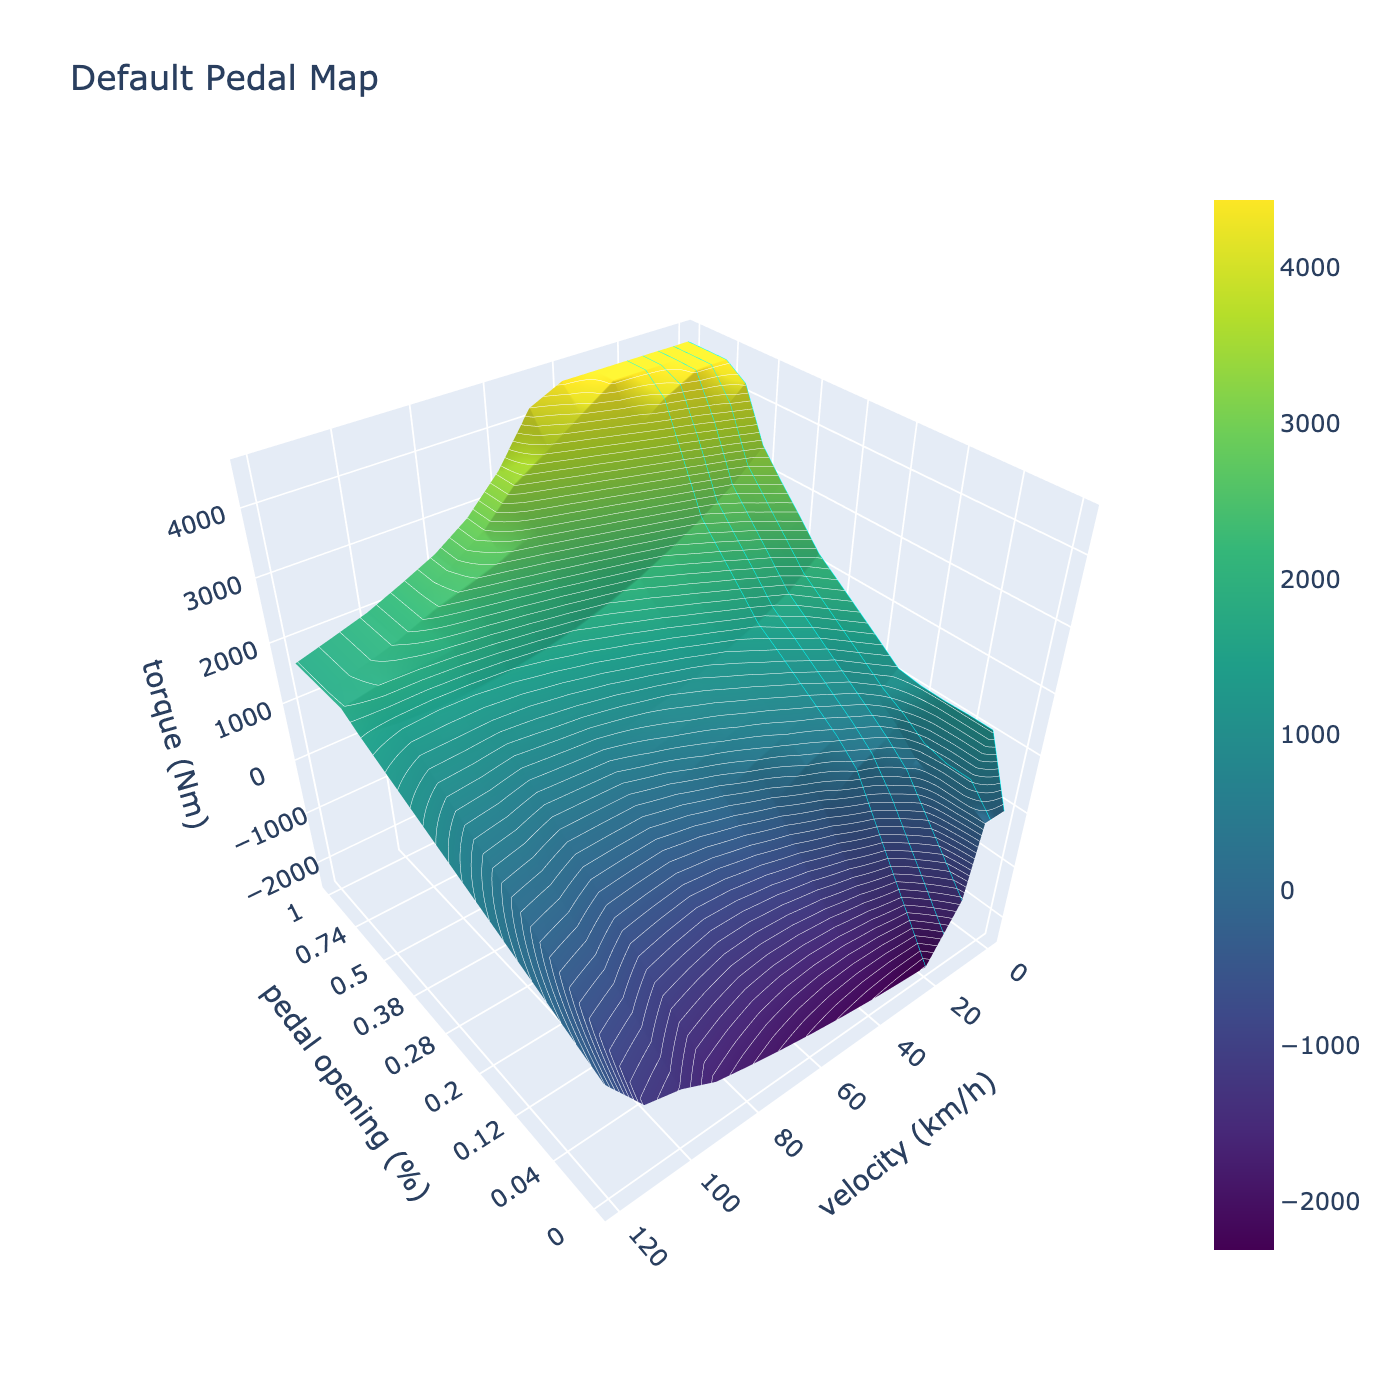
\includegraphics[width=\textwidth]{images/table_init.png}
		\caption{The ``Economic'' pedal map as the initial map}\label{fig:initial pedal map}
	\end{subfigure}
	\hfill
	\begin{subfigure}[b]{0.45\textwidth}
		\centering
		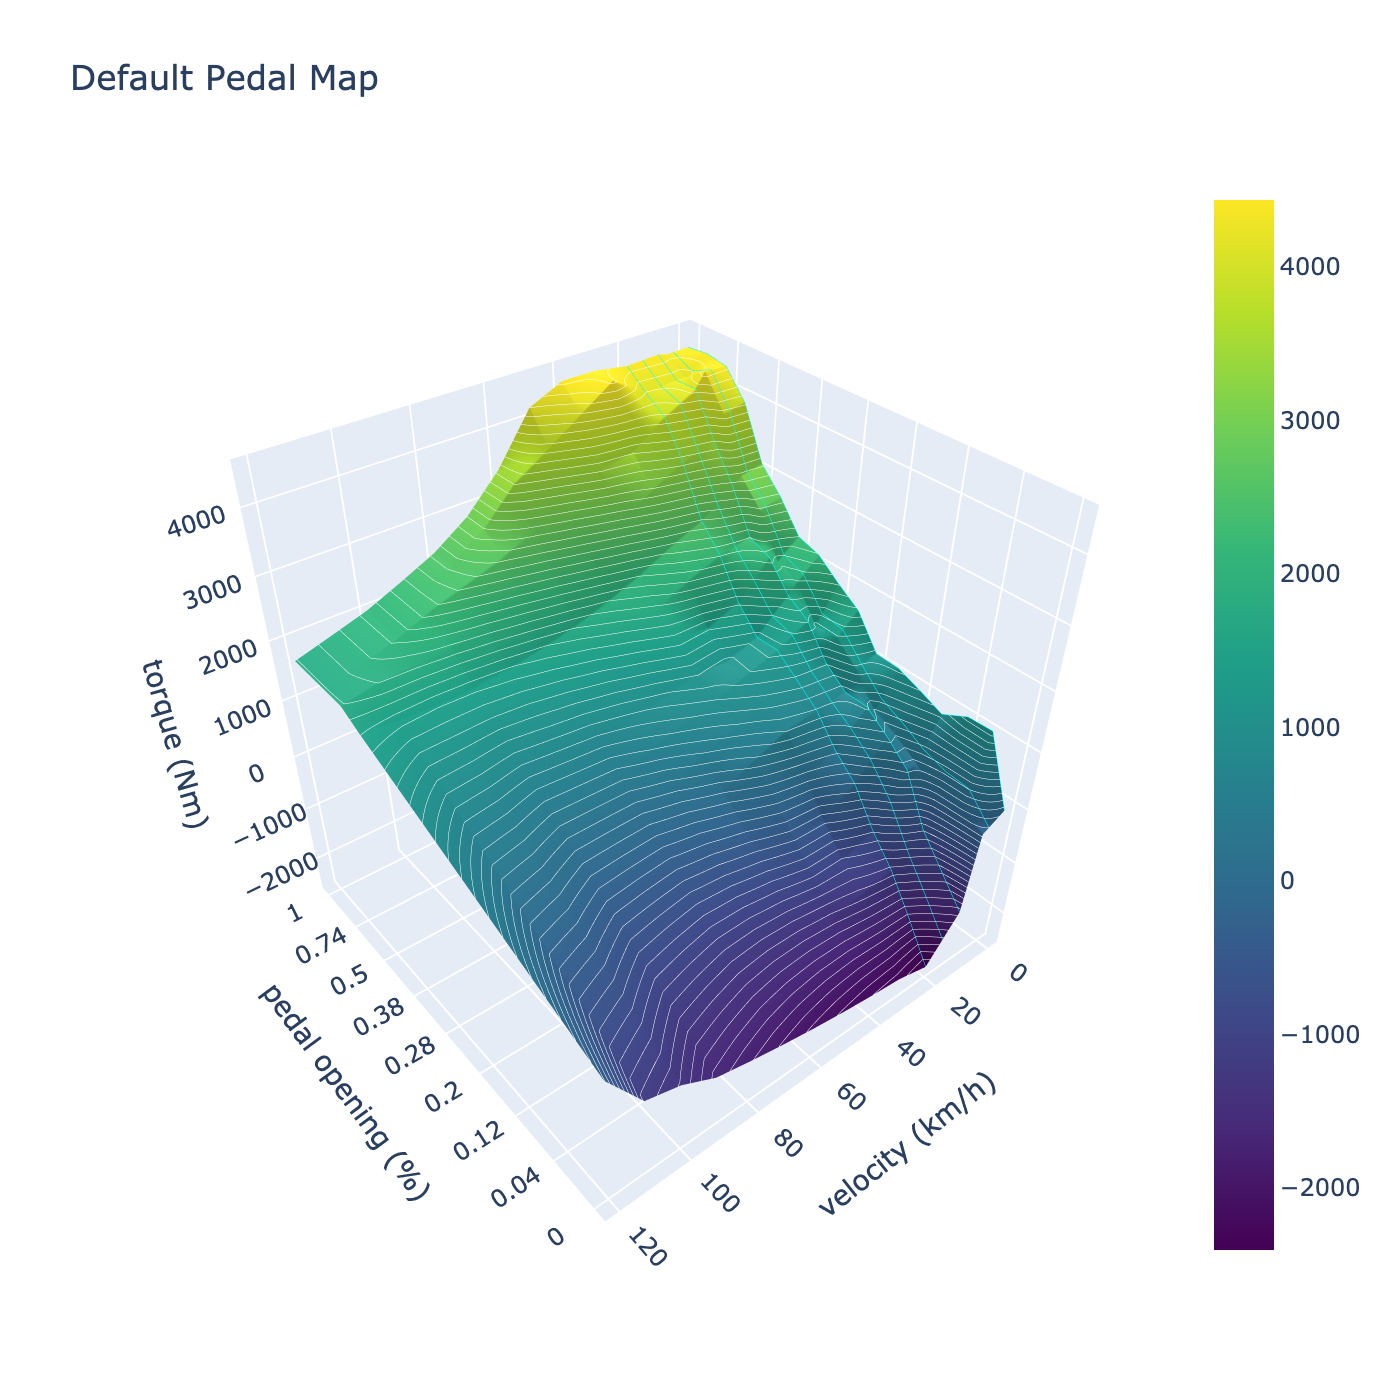
\includegraphics[width=\textwidth]{images/table_final.png}
		\caption{The dynamic pedal map}\label{fig:dynamic pedal map}
	\end{subfigure}
	\caption{\label{fig:pedal map} A pedal map is a 2d mapping table which outputs the torque request given a pedal opening under a certain vehicle speed. (a) The ``Economic'' pedal map is used as initial pedal map by the agent. (b) The pedal map is dynamically modified by the agent during driving conditioned on the vehicle speed and driver operation.}
\end{figure}

The pedal map is a two-dimensional table which outputs the torque request to the electric motor for a given acceleration pedal opening and a certain vehicle speed. It's a static map for a regular powertrain controller, as depicted in Fig.\@\ref{fig:initial pedal map}. The requested torque, once exerted by the electric motor, is proportional to teh vehicle acceleration. It's usually acquired by vehicle calibration during the pre-development of the EV model. A calibration engineer will generate different pedal maps by testing drives on proving ground or real road and determine table items empirically and by experimental validation. The different pedal maps will correspond to different driving styles which are provided as features to the customers, such as ``Normal'', ``Sport'' or ``Economic''. The customers will choose a pedal map through a vehicle HMI to match their driving style requirements. We select the ``Economic'' pedal map as the default initial pedal map for the agent and check how much the agent can further improve the energy efficiency. The pedal map increases monotonically with the acceleration pedal opening, while decreasing monotonically with the vehicle speed. The maximal torque request occurs when the vehicle starts off and the drive steps on the pedal with full throttle. The map region with low speed ($\leq10kmph$) and negligible pedal openings has the largest the negative torque request, which corresponds to motor in reverse, i.e.\ strong regenerative braking. These are all by design.

When the agent change the torque request for a given range of vehicle speeds under a give pedal opening, the corresponding region of the pedal map will be changed by $\Delta\tau$. If the training occurs on a urban road, we can see the low speed region under 60 kmph is changed as depicted in Fig.\ref{fig:dynamic pedal map}. The resulting pedal map is the sum of the initial map and integration of the action up to the current moment. In our experiment the agent is allowed to change the items all over the map region, which allows implicitly the exploitation of the regenerative braking.

\section{Method}\label{sec:method}

Once the design choice for the state, action, and reward are made, we apply the standard reinforcment learning, see Fig.\@\ref{fig:policy gradient}. We use a customized Deep Deterministic Policy Gradient algorithm \parencite{lillicrap15:_contin} due to its sample efficiency and continuous action space. The implementation is based on \parencite{keras20:DDPG}. During training, both the critic and the actor are updated with gradient descent by the reward signal, while for inference only the actor is required. Both the reward function $\mathcal{R}_a^s$ which generates the energy consumption and the system dynamic $\mathcal{P}_{ss'}^{a}$ which determines the state transition come from the real world. During training we keep a replay buffer to take new observations and sample batches from it.

\begin{figure}[ht]
	\centering
	\def\svgwidth{0.8\columnwidth}
	\documentclass{standalone}
\usepackage{tikz}
\usetikzlibrary{shapes.geometric, shapes, arrows, positioning}

\begin{document}

\begin{tikzpicture}[
    node distance=3cm,
    thick,
    signal/.style={draw,thick,circle,fill=blue!20},
    process/.style={draw,thick,minimum width=2cm,minimum height=1cm,rounded corners,fill=yellow!20,inner sep=.3cm},
    multimodal/.style={circle split,draw,double,fill=blue!20},
    state/.style={multimodal, minimum size=2cm},
    action/.style={multimodal, minimum size=2cm},
    reward/.style={multimodal, minimum size=2cm},
    actor/.style={process, minimum size=1.5cm, text centered},
    critic/.style={process, minimum size=1.5cm, text centered},
]

% Actor-Critic components
\node[actor] (actor) {Actor};
\node[critic, right of=actor] (critic) {Critic};

% Agent's environment interaction
\node[state, above left of=actor, yshift=1cm] (state) {State \nodepart{lower} $s$};
\node[action, right of=state, xshift=1.5cm] (action) {Action \nodepart{lower} $a$};
\node[reward, right of=action, xshift=1.5cm] (reward) {Reward \nodepart{lower} $r$};
\node[state, right of=reward, xshift=1.5cm] (next_state) {Next State\nodepart{lower} $s'$};

% Arrows connecting the components
%\path[->] (state) edge [bend left=30] node[above, sloped] {Policy} (action);
\path[->] (action) edge node[above, sloped] {$\mathcal{R}_a^s$} (reward);
\path[->] (action) edge [bend left=30] node[above, sloped] {$\mathcal{P}_{ss'}^{a}$} (next_state);
\path[->] (next_state.90) edge [bend right=40] node[above, sloped] {Update} (state.45);

% Arrows connecting actor and critic
\path[->] (state) edge (actor);
\path[->] (state.225) edge [bend right=90] (critic.225);
\path[->] (actor) edge (action);
\path[->] (reward) edge (critic);
\path[->] (action) edge (critic);
\path[->] (next_state) edge (critic.0);
\path[->] (critic) edge node[above] {Policy} node[below] {Gradient}(actor);

% Data flow within the components
\path[->] (actor) edge [loop above] node[above] {Policy} (actor);
\path[->] (critic) edge [loop below] node[below] {Value} (critic);

\end{tikzpicture}

\end{document}

	\caption{\label{fig:rl_model} The policy gradient method}\label{fig:policy gradient}
\end{figure}

\subsection{Model}\label{sec:model}

The neural networks for the critic and actor are depicted in Fig.\@\ref{fig:actorcritic}. We choose basic multi-layer perceptrons (MLPs) for both the actor and critic network. The activation function for the output layer of the actor network is $\tanh$ function which squeezes the output to $\left[0,1\right)$. Fig.\@\ref{fig:critic} also shows the training of the actor and critic, while Fig.\@\ref{fig:actor} is for the inference.

\begin{figure}[ht]
	\centering
	\begin{subfigure}[b]{0.55\textwidth}
		\centering
		\def\svgwidth{\columnwidth}
		\documentclass[tikz,border=3mm]{standalone}
\usepackage{xargs}
\usetikzlibrary{positioning,fit,calc}
\begin{document}

\tikzset{%
   neuron missing/.style={
    draw=none,
    scale=2,
    text height=0.333cm,
    execute at begin node=\color{black}$\vdots$
  },
}

% The command \DrawNeuronalNetwork has a list as argument, each entry is a
% layer. each entry has the form
%  Layer name/number of nodes/color/missing node/label/symbolic number
% where
% * layer name is, well,  the name of the layer
% * number of nodes is the number of neurons in that layer (including the missing neuron)
% * color is the color of the layer
% * missing node denotes the index of the missing neuron
% * label denotes the label of the layer
% * symbolic number denotes the symbol that indicates how many neurons there are
% * node content
\newcommandx{\DrawNeuronalNetwork}[5][1=0,2=0,3=0,4=State]{
\xdef\nn{#1}
\xdef\Xoff{#2}
\xdef\Yoff{#3}
\xdef\Inp{#4}
\xdef\Xmax{0}
\foreach \Layer/\X/\Col/\Miss/\Lab/\Count/\Content [count=\Y] in {#5}
{\pgfmathsetmacro{\Xmax}{max(\X,\Xmax)}
 \xdef\Xmax{\Xmax}
 \xdef\Ymax{\Y}
}
\ifnum\pdfstrcmp{\Inp}{concat}=0
\else
  \node (\nn-state) at (\Yoff,\Xoff) [draw,minimum width=6em,minimum height=4em] {\Inp};
\fi
\foreach \Layer/\X/\Col/\Miss/\Lab/\Count/\Content [count=\Y] in {#5}
    { \node[anchor=south] at ({2*\Y+\Yoff},{\Xmax/2-0.5+\Xoff}) {\Layer};
      \foreach \m in {1,...,\X}
      {
        \ifnum\m=\Miss
          \node [neuron missing] (nn-\nn--\Y-\m) at ({2*\Y+\Yoff},{\X/2-\m+\Xoff}) {};
        \else
          \ifnum\m=\X
            \node [circle,fill=\Col!50,minimum size=1cm] (nn-\nn-\Y-\m) at ({2*\Y+\Yoff},{\X/2-\m+\Xoff}) {\Content};
          \else
            \node [circle,fill=\Col!50,minimum size=1cm] (nn-\nn-\Y-\m) at ({2*\Y+\Yoff},{\X/2-\m+\Xoff}) {\m};
          \fi
          \ifnum\Y=1
          \else
            \pgfmathtruncatemacro{\LastY}{\Y-1}
            \foreach \Z in {1,...,\LastX}
            {
              \ifnum\Z=\LastMiss
              \else
                \draw[->] (nn-\nn-\LastY-\Z) -- (nn-\nn-\Y-\m);
              \fi
            }
          \fi
        \fi
        \ifnum\pdfstrcmp{\Inp}{concat}=0
          \ifnum\Y=1
            \ifnum\m=\X
              \foreach \Z in {1,...,5}
              {
                \ifnum\Z=4
                \else
                  \draw[->] [overlay] (nn-1-3-\Z) -- (nn-\nn-\Y-\m);
                  \draw[->] [overlay] (nn-2-2-\Z) -- (nn-\nn-\Y-\m);
                \fi
              }
            \else
              \ifnum\m=\Miss
              \else
                \foreach \Z in {1,...,5}
                {
                  \ifnum\Z=4
                  \else
                    \draw[->] [overlay] (nn-1-3-\Z) -- (nn-\nn-\Y-\m);
                    \draw[->] [overlay] (nn-2-2-\Z) -- (nn-\nn-\Y-\m);
                  \fi
                }
              \fi
            \fi
          \else
          \fi
        \else
          \ifnum\Y=1
            \ifnum\m=\X
              \draw [overlay] (nn-\nn-\Y-\m) -- (\nn-state);
            \else
              \ifnum\m=\Miss
              \else
                \draw [overlay] (nn-\nn-\Y-\m) -- (\nn-state);
              \fi
            \fi
          \else
          \fi
        \fi
      }
      \xdef\LastMiss{\Miss}
      \xdef\LastX{\X}
    }
}
\begin{tikzpicture}[x=1.5cm, y=1.5cm, >=stealth,font=\sffamily,nodes={align=center}]
\begin{scope}[local bounding box=T]
  \begin{scope}[local bounding box=NN]
   \DrawNeuronalNetwork[1][6][0][state]{State Input/5/green/4/inp1//600,
     Hidden 1/5/blue/4/h1//16,
     Hidden 2/5/cyan/4/h2//32}
   \DrawNeuronalNetwork[2][0][2][action]{Action Input/5/green/4/inp2//68,
     Hidden 3/5/yellow/4/out//32}
   \DrawNeuronalNetwork[3][3][8][concat]{Hidden 4/5/orange/4/out//64,
     Hidden 5/5/blue/4/h1//64,
     Output/1/green/0/output//1}
  \end{scope}
  \path (NN.south) node[below]{Estimated parameter\\ $\theta$};
  \path (nn-3-3-1.east) -- node[above]{Action value\\ $q_{\pi_{\theta}}(s,a)$}++ (4em,0);
 \end{scope}
 \node[fit=(T),label={[anchor=north west]north west:Critic},inner sep=1em,draw]
  (TF){};
 \node[below=3em of TF,draw,inner sep=1em] (Env) {Environment};
 \node[below=3em of TF,draw,inner sep=1em, right = 3 of Env] (Actor) {Actor};
 \node[circle, fill, inner sep=2pt] at (Env.170) (rt) {};
 \node[circle, fill, inner sep=2pt] at (Env.190) (st) {};
 \draw[<-] (TF.200) -- ++ (-2em,0) |- (Env.170) node[pos=0.45,right]{$r_t$};
 \draw[<-] (1-state) -- ++ (-8em,0) |- (Env.190) node[pos=0.45,left]{$s_t$};
 \draw[->] (nn-3-3-1.east) -- ++ (7em,0) |- node [above, pos=0.85]{Policy Gradient} (Actor) -- node[pos=0.5, circle, fill, inner sep=2pt] (Action) {} node[above,pos=0.4]{{$a_t$}} (Env);
 \coordinate (A) at ($ (Action) + (0, 0.5) $);
 %\coordinate let \p1=(Env.180), \p2=(Env.160) in (A) at ($ (Action) + (0, 0.5) $);
 \draw[<-]  let \p1=(Env.180), \p2=(Env.160) in (2-state) -- ++ (-8em,0) |- ($(Action) + (0, \y2-\y1) + (0, \y2-\y1)$) node[pos=0.2,left]{$a_t$} -- (Action);
 %\draw[<-] (2-state) -- ++ (-8em,0) |- (A) node[pos=0.2,left]{$a_t$} -- (Action);
\end{tikzpicture}
\end{document}

		\caption{\label{fig:critic} The critic}
	\end{subfigure}
	\hfill
	\begin{subfigure}[b]{0.4\textwidth}
		\centering
		\def\svgwidth{\columnwidth}
		\documentclass[tikz,border=3mm]{standalone}
\usetikzlibrary{positioning,fit}
\begin{document}

\tikzset{%
   neuron missing/.style={
    draw=none,
    scale=2,
    text height=0.333cm,
    execute at begin node=\color{black}$\vdots$
  },
}

% The command \DrawNeuronalNetwork has a list as argument, each entry is a
% layer. each entry has the form
%  Layer name/number of nodes/color/missing node/label/symbolic number
% where
% * layer name is, well,  the name of the layer
% * number of nodes is the number of neurons in that layer (including the missing neuron)
% * color is the color of the layer
% * missing node denotes the index of the missing neuron
% * label denotes the label of the layer
% * symbolic number denotes the symbol that indicates how many neurons there are
% * node content
\newcommand{\DrawNeuronalNetwork}[2][]{
\xdef\Xmax{0}
\foreach \Layer/\X/\Col/\Miss/\Lab/\Count/\Content [count=\Y] in {#2}
{\pgfmathsetmacro{\Xmax}{max(\X,\Xmax)}
 \xdef\Xmax{\Xmax}
 \xdef\Ymax{\Y}
}
\foreach \Layer/\X/\Col/\Miss/\Lab/\Count/\Content [count=\Y] in {#2}
    {\node[anchor=south] at ({2*\Y},{\Xmax/2+0.1}) {\Layer};
      \foreach \m in {1,...,\X}
      {
        \ifnum\m=\Miss
          \node [neuron missing] (neuron-\Y-\m) at ({2*\Y},{\X/2-\m}) {};
        \else
          \ifnum\m=\X
            \node [circle,fill=\Col!50,minimum size=1cm] (neuron-\Y-\m) at ({2*\Y},{\X/2-\m}) {\Content};
          \else
            \node [circle,fill=\Col!50,minimum size=1cm] (neuron-\Y-\m) at ({2*\Y},{\X/2-\m}) {\m};
          \fi
          \ifnum\Y=1
          \else
            \pgfmathtruncatemacro{\LastY}{\Y-1}
            \foreach \Z in {1,...,\LastX}
            {
              \ifnum\Z=\LastMiss
              \else
                \draw[->] (neuron-\LastY-\Z) -- (neuron-\Y-\m);
              \fi
            }
          \fi
        \fi
        \ifnum\Y=1
          \ifnum\m=\X
            \draw [overlay] (neuron-\Y-\m) -- (state);
          \else
            \ifnum\m=\Miss
            \else
              \draw [overlay] (neuron-\Y-\m) -- (state);
            \fi
          \fi
        \else
        \fi
      }
      \xdef\LastMiss{\Miss}
      \xdef\LastX{\X}
    }
}
\begin{tikzpicture}[x=1.5cm, y=1.5cm, >=stealth,font=\sffamily,nodes={align=center}]
 \begin{scope}[local bounding box=T]
  \path  node[draw,minimum width=6em,minimum height=4em] (state) {State};
  \begin{scope}[local bounding box=NN]
   \DrawNeuronalNetwork{Input Layer/5/green/4/inp//600,
     Hidden Layer 1/5/blue/4/h1//256,
     Hidden Layer 2/5/cyan/4/h2//256,
     Output Layer/4/red/3/out//68}
  \end{scope}
  \path (NN.south) node[below]{Estimated parameter\\ $\theta$};
  \path (NN.east) -- node[above]{Policy\\ $\Pi(\theta,a)$}++ (4em,0);
 \end{scope}
 \node[fit=(T),label={[anchor=north west]north west:Actor},inner sep=1em,draw]
  (TF){};
 \node[below=3em of TF,draw,inner sep=1em] (Env) {Environment};
 \draw[<-] (TF.200) -- ++ (-1em,0) |- (Env.160) node[pos=0.45,right]{$r_t$};
 \draw[<-] (TF.180) -- ++ (-2em,0) |- (Env.180) node[pos=0.45,left]{$s_t$};
 \draw[->] (NN.east) -- ++ (7em,0)node[right]{$a_t$} |- (Env);
\end{tikzpicture}
\end{document}

		\caption{\label{fig:actor} The actor}
	\end{subfigure}
	\caption{The actor and critic network. The numbers in the neurons stand for the dimension in the layers, see sec.\@\ref{sec:setup}.}\label{fig:actorcritic}
\end{figure}


%\begin{figure}[ht]
%	\centering
%	\def\svgwidth{0.45\columnwidth}
%	\documentclass[tikz,border=3mm]{standalone}
\usepackage{xargs}
\usetikzlibrary{positioning,fit,calc}
\begin{document}

\tikzset{%
   neuron missing/.style={
    draw=none,
    scale=2,
    text height=0.333cm,
    execute at begin node=\color{black}$\vdots$
  },
}

% The command \DrawNeuronalNetwork has a list as argument, each entry is a
% layer. each entry has the form
%  Layer name/number of nodes/color/missing node/label/symbolic number
% where
% * layer name is, well,  the name of the layer
% * number of nodes is the number of neurons in that layer (including the missing neuron)
% * color is the color of the layer
% * missing node denotes the index of the missing neuron
% * label denotes the label of the layer
% * symbolic number denotes the symbol that indicates how many neurons there are
% * node content
\newcommandx{\DrawNeuronalNetwork}[5][1=0,2=0,3=0,4=State]{
\xdef\nn{#1}
\xdef\Xoff{#2}
\xdef\Yoff{#3}
\xdef\Inp{#4}
\xdef\Xmax{0}
\foreach \Layer/\X/\Col/\Miss/\Lab/\Count/\Content [count=\Y] in {#5}
{\pgfmathsetmacro{\Xmax}{max(\X,\Xmax)}
 \xdef\Xmax{\Xmax}
 \xdef\Ymax{\Y}
}
\ifnum\pdfstrcmp{\Inp}{concat}=0
\else
  \node (\nn-state) at (\Yoff,\Xoff) [draw,minimum width=6em,minimum height=4em] {\Inp};
\fi
\foreach \Layer/\X/\Col/\Miss/\Lab/\Count/\Content [count=\Y] in {#5}
    { \node[anchor=south] at ({2*\Y+\Yoff},{\Xmax/2-0.5+\Xoff}) {\Layer};
      \foreach \m in {1,...,\X}
      {
        \ifnum\m=\Miss
          \node [neuron missing] (nn-\nn--\Y-\m) at ({2*\Y+\Yoff},{\X/2-\m+\Xoff}) {};
        \else
          \ifnum\m=\X
            \node [circle,fill=\Col!50,minimum size=1cm] (nn-\nn-\Y-\m) at ({2*\Y+\Yoff},{\X/2-\m+\Xoff}) {\Content};
          \else
            \node [circle,fill=\Col!50,minimum size=1cm] (nn-\nn-\Y-\m) at ({2*\Y+\Yoff},{\X/2-\m+\Xoff}) {\m};
          \fi
          \ifnum\Y=1
          \else
            \pgfmathtruncatemacro{\LastY}{\Y-1}
            \foreach \Z in {1,...,\LastX}
            {
              \ifnum\Z=\LastMiss
              \else
                \draw[->] (nn-\nn-\LastY-\Z) -- (nn-\nn-\Y-\m);
              \fi
            }
          \fi
        \fi
        \ifnum\pdfstrcmp{\Inp}{concat}=0
          \ifnum\Y=1
            \ifnum\m=\X
              \foreach \Z in {1,...,5}
              {
                \ifnum\Z=4
                \else
                  \draw[->] [overlay] (nn-1-3-\Z) -- (nn-\nn-\Y-\m);
                  \draw[->] [overlay] (nn-2-2-\Z) -- (nn-\nn-\Y-\m);
                \fi
              }
            \else
              \ifnum\m=\Miss
              \else
                \foreach \Z in {1,...,5}
                {
                  \ifnum\Z=4
                  \else
                    \draw[->] [overlay] (nn-1-3-\Z) -- (nn-\nn-\Y-\m);
                    \draw[->] [overlay] (nn-2-2-\Z) -- (nn-\nn-\Y-\m);
                  \fi
                }
              \fi
            \fi
          \else
          \fi
        \else
          \ifnum\Y=1
            \ifnum\m=\X
              \draw [overlay] (nn-\nn-\Y-\m) -- (\nn-state);
            \else
              \ifnum\m=\Miss
              \else
                \draw [overlay] (nn-\nn-\Y-\m) -- (\nn-state);
              \fi
            \fi
          \else
          \fi
        \fi
      }
      \xdef\LastMiss{\Miss}
      \xdef\LastX{\X}
    }
}
\begin{tikzpicture}[x=1.5cm, y=1.5cm, >=stealth,font=\sffamily,nodes={align=center}]
\begin{scope}[local bounding box=T]
  \begin{scope}[local bounding box=NN]
   \DrawNeuronalNetwork[1][6][0][state]{State Input/5/green/4/inp1//600,
     Hidden 1/5/blue/4/h1//16,
     Hidden 2/5/cyan/4/h2//32}
   \DrawNeuronalNetwork[2][0][2][action]{Action Input/5/green/4/inp2//68,
     Hidden 3/5/yellow/4/out//32}
   \DrawNeuronalNetwork[3][3][8][concat]{Hidden 4/5/orange/4/out//64,
     Hidden 5/5/blue/4/h1//64,
     Output/1/green/0/output//1}
  \end{scope}
  \path (NN.south) node[below]{Estimated parameter\\ $\theta$};
  \path (nn-3-3-1.east) -- node[above]{Action value\\ $q_{\pi_{\theta}}(s,a)$}++ (4em,0);
 \end{scope}
 \node[fit=(T),label={[anchor=north west]north west:Critic},inner sep=1em,draw]
  (TF){};
 \node[below=3em of TF,draw,inner sep=1em] (Env) {Environment};
 \node[below=3em of TF,draw,inner sep=1em, right = 3 of Env] (Actor) {Actor};
 \node[circle, fill, inner sep=2pt] at (Env.170) (rt) {};
 \node[circle, fill, inner sep=2pt] at (Env.190) (st) {};
 \draw[<-] (TF.200) -- ++ (-2em,0) |- (Env.170) node[pos=0.45,right]{$r_t$};
 \draw[<-] (1-state) -- ++ (-8em,0) |- (Env.190) node[pos=0.45,left]{$s_t$};
 \draw[->] (nn-3-3-1.east) -- ++ (7em,0) |- node [above, pos=0.85]{Policy Gradient} (Actor) -- node[pos=0.5, circle, fill, inner sep=2pt] (Action) {} node[above,pos=0.4]{{$a_t$}} (Env);
 \coordinate (A) at ($ (Action) + (0, 0.5) $);
 %\coordinate let \p1=(Env.180), \p2=(Env.160) in (A) at ($ (Action) + (0, 0.5) $);
 \draw[<-]  let \p1=(Env.180), \p2=(Env.160) in (2-state) -- ++ (-8em,0) |- ($(Action) + (0, \y2-\y1) + (0, \y2-\y1)$) node[pos=0.2,left]{$a_t$} -- (Action);
 %\draw[<-] (2-state) -- ++ (-8em,0) |- (A) node[pos=0.2,left]{$a_t$} -- (Action);
\end{tikzpicture}
\end{document}

%	\caption{\label{fig:critic} The critic model in the training mode}
%	\label{fig:critic in training}
%\end{figure}
%\begin{figure}[ht]
%	\centering
%	\def\svgwidth{0.45\columnwidth}
%	\documentclass[tikz,border=3mm]{standalone}
\usetikzlibrary{positioning,fit}
\begin{document}

\tikzset{%
   neuron missing/.style={
    draw=none,
    scale=2,
    text height=0.333cm,
    execute at begin node=\color{black}$\vdots$
  },
}

% The command \DrawNeuronalNetwork has a list as argument, each entry is a
% layer. each entry has the form
%  Layer name/number of nodes/color/missing node/label/symbolic number
% where
% * layer name is, well,  the name of the layer
% * number of nodes is the number of neurons in that layer (including the missing neuron)
% * color is the color of the layer
% * missing node denotes the index of the missing neuron
% * label denotes the label of the layer
% * symbolic number denotes the symbol that indicates how many neurons there are
% * node content
\newcommand{\DrawNeuronalNetwork}[2][]{
\xdef\Xmax{0}
\foreach \Layer/\X/\Col/\Miss/\Lab/\Count/\Content [count=\Y] in {#2}
{\pgfmathsetmacro{\Xmax}{max(\X,\Xmax)}
 \xdef\Xmax{\Xmax}
 \xdef\Ymax{\Y}
}
\foreach \Layer/\X/\Col/\Miss/\Lab/\Count/\Content [count=\Y] in {#2}
    {\node[anchor=south] at ({2*\Y},{\Xmax/2+0.1}) {\Layer};
      \foreach \m in {1,...,\X}
      {
        \ifnum\m=\Miss
          \node [neuron missing] (neuron-\Y-\m) at ({2*\Y},{\X/2-\m}) {};
        \else
          \ifnum\m=\X
            \node [circle,fill=\Col!50,minimum size=1cm] (neuron-\Y-\m) at ({2*\Y},{\X/2-\m}) {\Content};
          \else
            \node [circle,fill=\Col!50,minimum size=1cm] (neuron-\Y-\m) at ({2*\Y},{\X/2-\m}) {\m};
          \fi
          \ifnum\Y=1
          \else
            \pgfmathtruncatemacro{\LastY}{\Y-1}
            \foreach \Z in {1,...,\LastX}
            {
              \ifnum\Z=\LastMiss
              \else
                \draw[->] (neuron-\LastY-\Z) -- (neuron-\Y-\m);
              \fi
            }
          \fi
        \fi
        \ifnum\Y=1
          \ifnum\m=\X
            \draw [overlay] (neuron-\Y-\m) -- (state);
          \else
            \ifnum\m=\Miss
            \else
              \draw [overlay] (neuron-\Y-\m) -- (state);
            \fi
          \fi
        \else
        \fi
      }
      \xdef\LastMiss{\Miss}
      \xdef\LastX{\X}
    }
}
\begin{tikzpicture}[x=1.5cm, y=1.5cm, >=stealth,font=\sffamily,nodes={align=center}]
 \begin{scope}[local bounding box=T]
  \path  node[draw,minimum width=6em,minimum height=4em] (state) {State};
  \begin{scope}[local bounding box=NN]
   \DrawNeuronalNetwork{Input Layer/5/green/4/inp//600,
     Hidden Layer 1/5/blue/4/h1//256,
     Hidden Layer 2/5/cyan/4/h2//256,
     Output Layer/4/red/3/out//68}
  \end{scope}
  \path (NN.south) node[below]{Estimated parameter\\ $\theta$};
  \path (NN.east) -- node[above]{Policy\\ $\Pi(\theta,a)$}++ (4em,0);
 \end{scope}
 \node[fit=(T),label={[anchor=north west]north west:Actor},inner sep=1em,draw]
  (TF){};
 \node[below=3em of TF,draw,inner sep=1em] (Env) {Environment};
 \draw[<-] (TF.200) -- ++ (-1em,0) |- (Env.160) node[pos=0.45,right]{$r_t$};
 \draw[<-] (TF.180) -- ++ (-2em,0) |- (Env.180) node[pos=0.45,left]{$s_t$};
 \draw[->] (NN.east) -- ++ (7em,0)node[right]{$a_t$} |- (Env);
\end{tikzpicture}
\end{document}

%	\caption{\label{fig:actor} The actor in the inference mode}
%	\label{fig:actor in inference}
%\end{figure}


\subsection{Experimental Setup}\label{sec:setup}

The training setup is important for the agent to learn a good policy. As a basic requirement for reinforcement learning, the training should be episodic. We first choose a short episode with a target speed profile as depicted in Fig.\@\ref{fig:speed profile for traning}, while the vehicle is simply driven forward. From a standstill, the vehicle needs to be accelerated to a maximal speed of around 17kmph. After deceleration it return to its standstill state. An upperbound and lowerbound is set for allowed maximal deviation from the desired target speed. If the actual speed is out of the bound for longer than three seconds, the test episode is invalid or should be interrupted prematurely and the data is abandoned. The test is carried out on a proving ground with no traffic or pedestrian. With this simple speed profile we expect the agent to learn the basic policy of acceleration and deceleration and thus be prepared for more complex scenarios.

\begin{figure}
	\begin{minipage}[b]{0.5\linewidth}
		\centering
		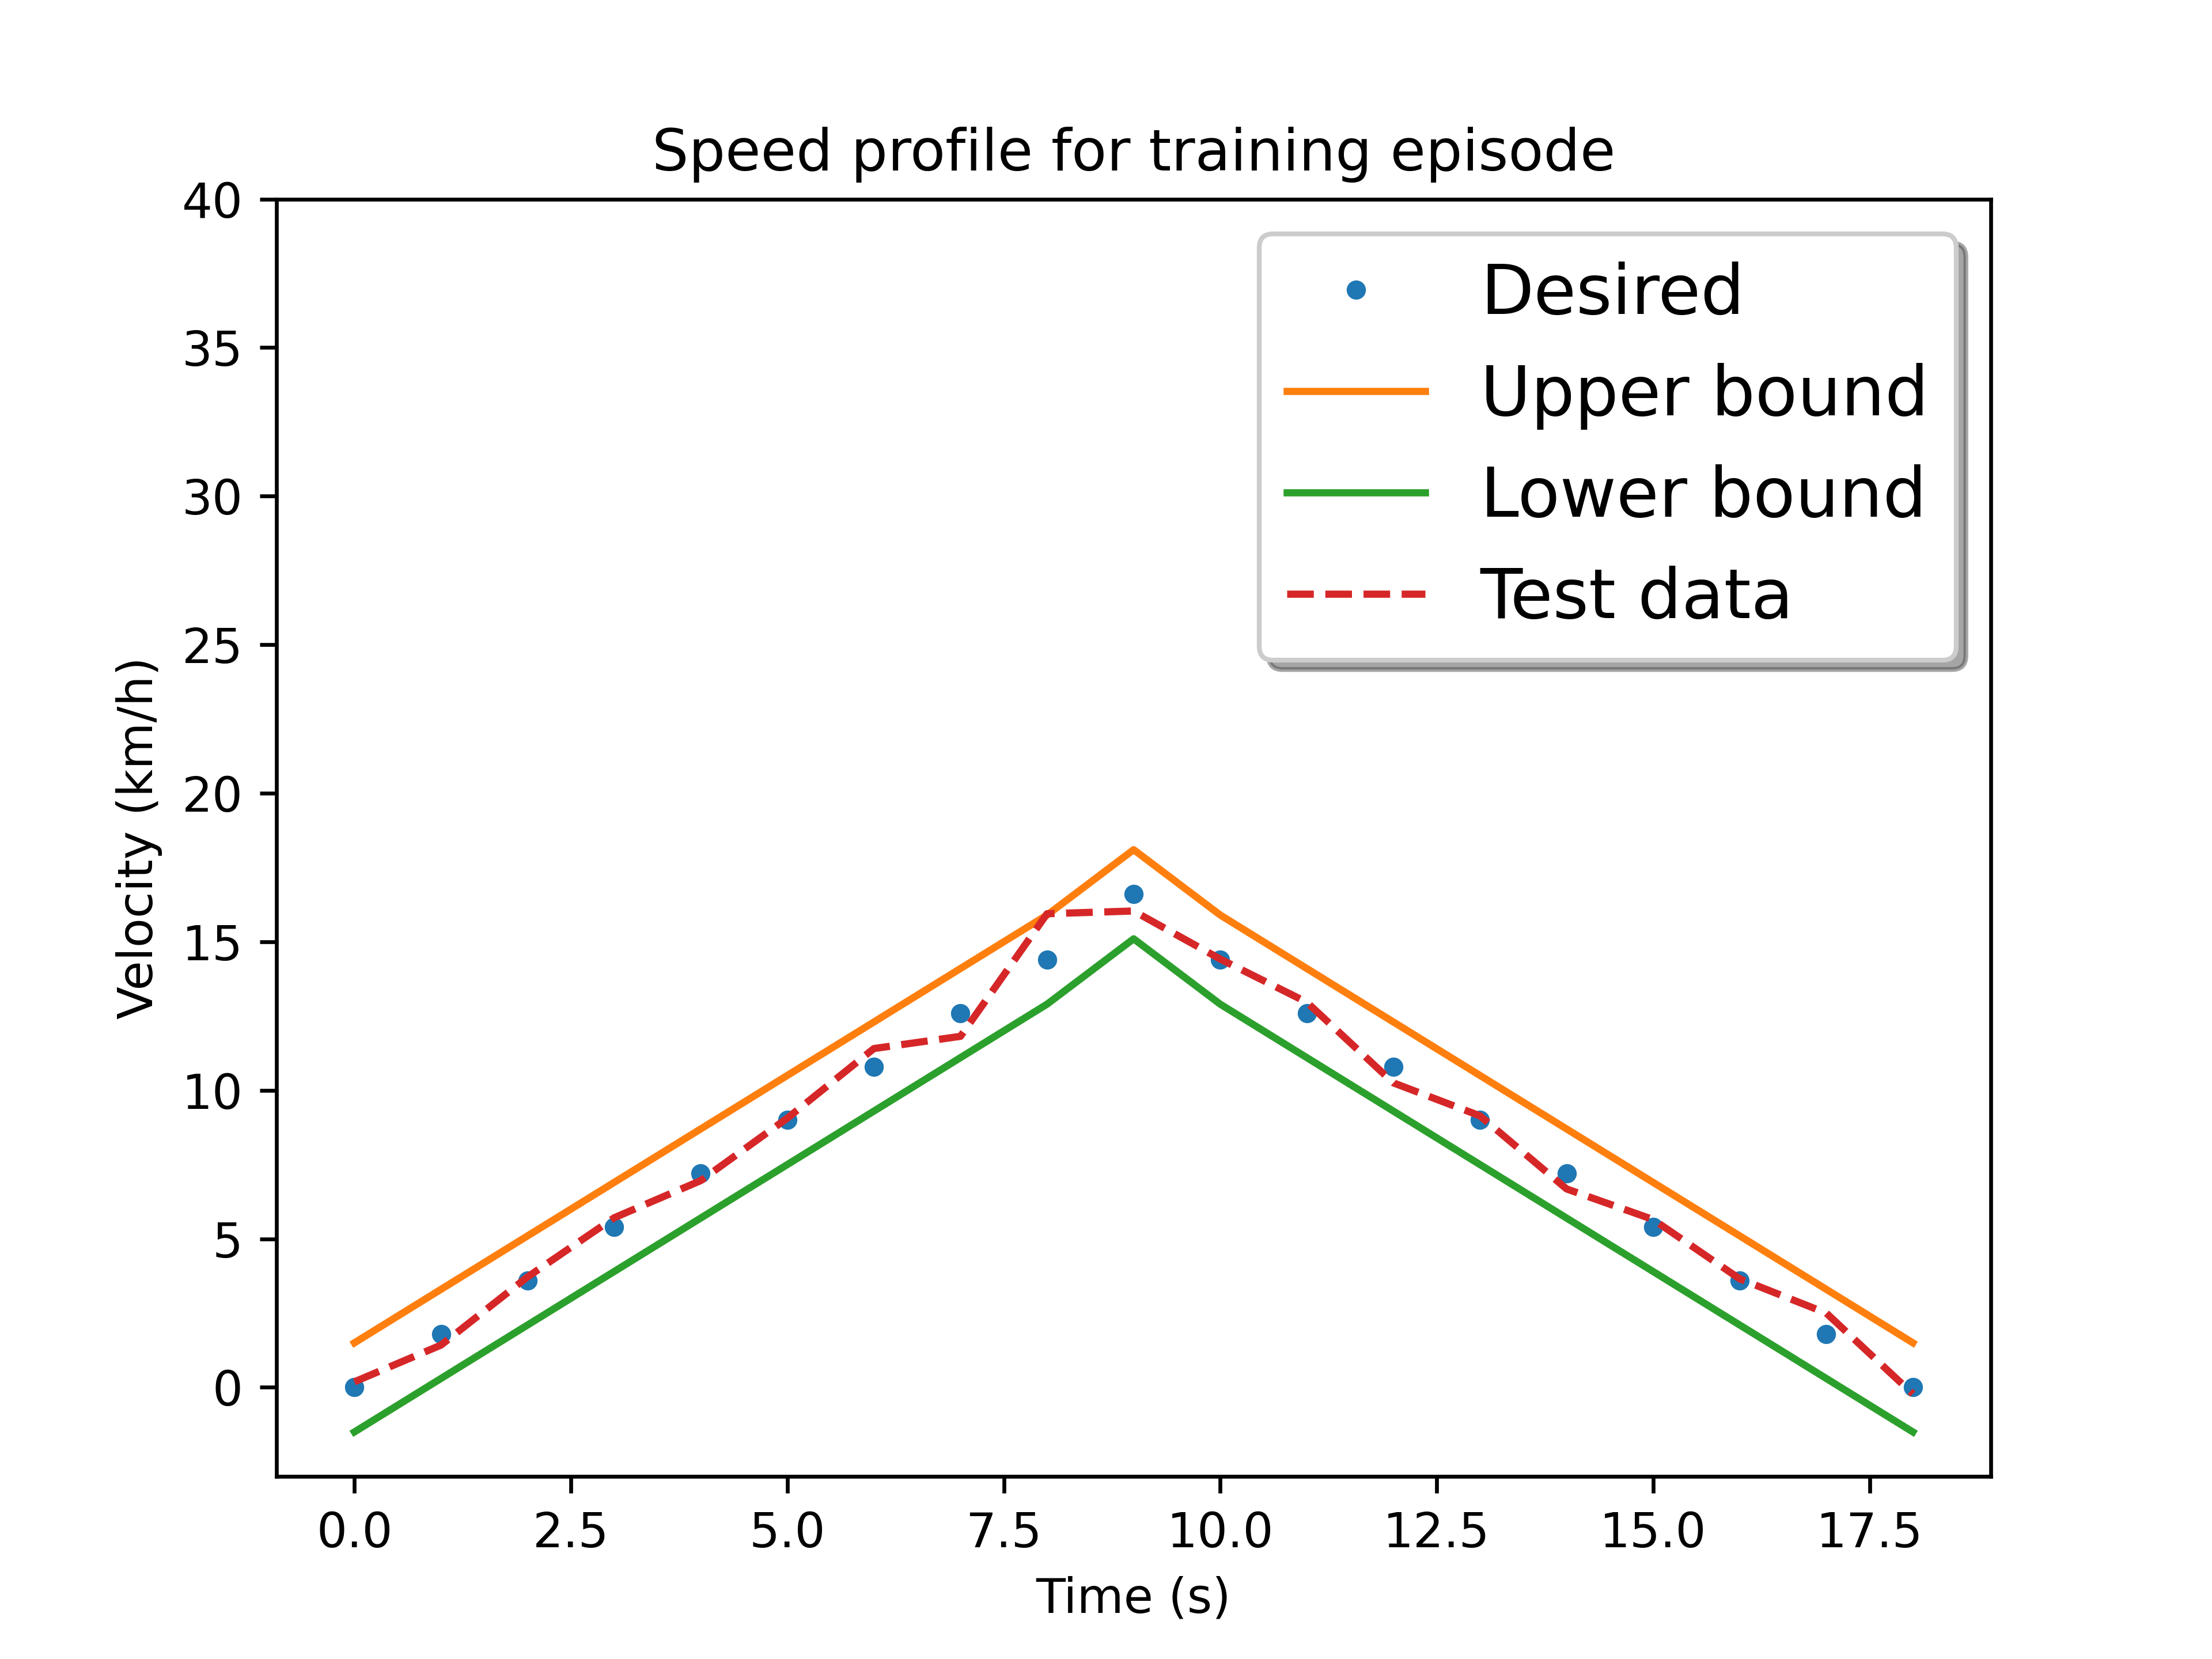
\includegraphics[scale=0.5]{images/speed_profile.png}
		\captionof{figure}{\label{fig:speed profile for traning} Speed profile of the episode used for training}
	\end{minipage}
	\quad
	\begin{minipage}[b]{0.45\linewidth}
		\centering
		\begin{tabular}{c c c c c}
			\toprule
			$t$ & $s_{t}$                               & $a_t$         & $r_t$                    & $s'_t$                                   \\
			\cmidrule(r){1-1} \cmidrule(r){2-4} \cmidrule{5-5}
			$T$ & $V_1$, $A_1$, $B_1$                   &               & $U_{1}$, $I_{1}$         & $V'_1$, $A'_1$, $B'_1$                   \\
			    & \ldots                                &               & \ldots                   & \ldots                                   \\
			    & $V_{i_{1}}$, $A_{i_{1}}$, $B_{i_{1}}$ &               & $U_{i_{1}}$, $I_{i_{1}}$ & $V'_{i_{1}}$, $A'_{i_{1}}$, $B'_{i_{1}}$ \\
			    & \ldots                                &               & \ldots                   & \ldots                                   \\
			    & $V_{i_{l}}$, $A_{i_l}$, $B_{i_l}$     &               & $U_{i_{l}}$, $I_{i_{l}}$ & $V'_{i_{l}}$, $A'_{i_{l}}$, $B'_{i_{l}}$ \\
			    & \ldots                                &               & \ldots                   & \ldots                                   \\
			    & $V_K$, $A_K$, $B_K$                   & $\Delta \tau$ & $U_K$, $I_K$             & $V'_K$, $A'_K$, $B'_K$                   \\
			\bottomrule
		\end{tabular}
		\captionof{table}{\label{tab:quadruple} Record: A quartic tuple with a timestamp $T$}
	\end{minipage}\hfill
\end{figure}

\subsubsection{Record}\label{sec:record}

The data in the reinforcement learning model are shown in Tab.\@\ref{tab:quadruple}. The definitions and special notes:

\begin{description}
	\item[State] Since DDPG is not a sequential model, we take the array of $K$ subsequent observations of $(V,A,B)$ as state $s_{t}=(V_{1},A_{1},B_{1},\ldots,V_{K},A_{K},B_{K})$, where each observation is a CAN frame. In the experiment, $K=30$, which amounts to 1.5 seconds of observation for the frame rate at 20 Hz, thus the state dimension for input layers in Fig.\@\ref{fig:actorcritic} is 90. The actor outputs the action $\Delta\tau$ given the state array.

	\item[Action] The dimension of the pedal map in our experiment is $17\times 21$, where the columns axis corresponds to acceleration pedal opening from 0\% to 100\% and the rows axis to the speed range of 0 kmph to 100 kmph. The torque request of the ``Economic'' map ranges from around -2 kNm to 4.4 kNm. While the whole region of the pedal map can be changed by action, it's usually not necessary. Since the acceleration of the vehicle is limited in the usual driving senarios, we choose the action dimension to be $17\times 4=68$, namely 4 rows of the map depending on the observed speed values in the state.  This corresponds to a maximal acceleration of 0.37$g$ (or $3.7m/s^{2}$). While the output of the actor $a_{t}=\Delta\tau$ will change any rows of the pedal map depending on the the speed of the vehicle, the same actor network is used, which means the agent share the same policy for changing the torque request under different speeds. The sharing of same network for different observation reduces the model capacity as well as computation.

	\item[Reward] $r_{t}=\Sigma_{k=1}^{K}(U_{k}\cdot I_{k})$.

	\item[Causality] Care needs to be taken regarding causality of the signal. Since $\Delta\tau$ is computed by the agent after receiving the state array, it will only impact the driving after the pedal map has been written into the VCU flash memory and the eletric motor exerts the requested torque physically, which means only the energy consumption after the torque exertion should be attributed to this action as reward. After receiving the sequence of the raw observations, caching and reordering are necessary. For example, the reward $r_{t}$ for the current action $a_{t}$ comes from the next 1.5 seconds, while the reward in the current observation should be attributed to the last action. Therefore in the next 1.5 seconds only the reward is collected after the action is carried out, which also ensures the next state $s'_{t} (s_{t+1})$ is stable and caused by $a_{t}$. The scheduling of data collection in this way avoids the intererences of subsequent actions, states and rewards thus the signal causality which is crucial for the value estimation.

	\item[Loss tokens] In case of frame loss, we simply replace the missing data with null elements as loss tokens, which will be utilized for the agent as a learning signal for handling information loss.

	\item[Action clipping] Action clipping similar to target policy smoothing in TD3 \parencite{TD3:_addres_funct_approx_error_actor_critic_method} is used. For the sake of simplicity, we don't use the double-Q learning or delayed polciy updates. For each training drive, we reload the pedal map from the last drive as the initial map for the current drive. A torque change budget is defined, which should be multiplied by the action value, the $\tanh$ outputs of the actor, to be added to the current pedal map. In our experiment, the torque budget is 200 Nm. The pedal map is then clipped on the lower and upperbound around the initial pedal map of the current drive and further clipping on the allowed maximal torque request.

\end{description}

As a result, For every 3 seconds we get one quartic tuple in Tab.\@\ref{tab:quadruple} which is called a ``record'' and can be fed into the DDPG agent for inference or stored in the replay buffer for sampling batches during the training.

\subsubsection{Episode}\label{sec:episode}

For sequential models like RDPG \parencite{heess15:_memor}, a sequence of states, namely the history, needs to be fed into sequential neural networks. For this purpose, ``episodes'' will be stored in the replay buffer. An episode is a consecutive sequence of records with a start and an end state $e_T=[(s_1,a_1,r_1),\ldots,(s_{N},a_{N},r_{N})]$. Similarly to the data handling for the DDPG agent, null elements are inserted in the episodes as loss tokens if observations are missing, which happens quite often for over-the-air (OTA) vehicle communication interface. In general, episodes have different sequence length, since the termination of an episode could mean reaching the destination with different speeds or events. Therefore the replay buffer for episodes is ususally ragged.

\subsection{Training}\label{sec:training}

When an episode starts, only inference will be done while collecting the states, actions and rewards until the episode ends. Then only after that, the actor and critic are updated with batch sampling from the replay buffer.

As can be seen in Fig.\@\ref{fig:Agent_Powertrain}, the environment of the reinforcement learning model include both the vehicle on the road and the driver. If we fix the same vehicle and test drive on the same site, we expect both to be stationary. We fix the driver for the test as well, since each driver is expected to have fixed driving style. Therefore we assume the driving style also to be stationary. However, since each driver has his own driving style, we monitor the driving style of the driver for analysis of its impact on the overall EOSEV system.

\subsubsection{Driving style}\label{sec:driving style}

\begin{figure}[htbp]
	\centering
	\begin{subfigure}[b]{0.45\textwidth}
		\centering
		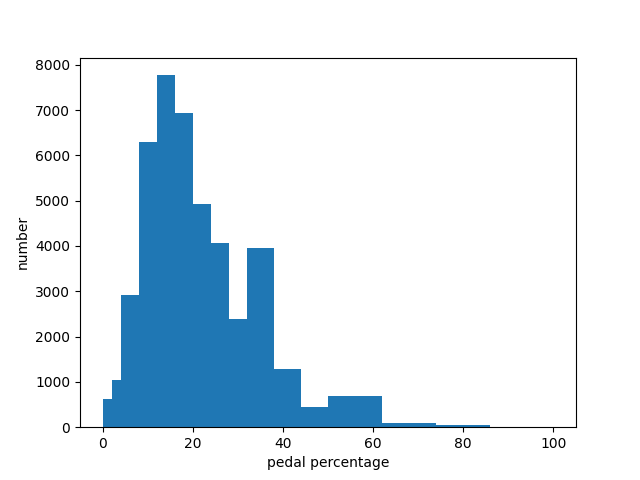
\includegraphics[width=\textwidth]{images/no-ai-driving-style.png}
		\caption{Baseline style without agent}\label{fig:driving style without agent}
	\end{subfigure}
	\hfill
	\begin{subfigure}[b]{0.45\textwidth}
		\centering
		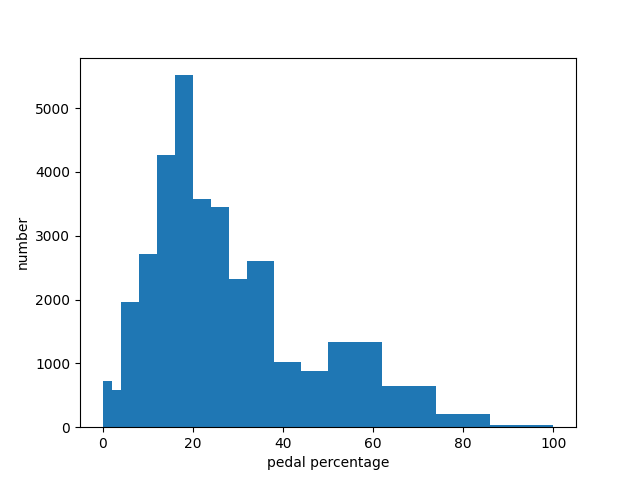
\includegraphics[width=\textwidth]{images/ai-driving-style.png}
		\caption{Distribution with agent switched on}\label{fig:driving style with agent}
	\end{subfigure}\caption{\label{fig:driving styles} Driving styles as distribution of acceleration pedal openings.}
\end{figure}

For each episode we can calculate the distribution of the pedal openings and denote it as driving style. As the baseline we calculate the average distribution of over 70 episdoes with the same driver, vehicle and configurations with the agent switched off. Fig.\@\ref{fig:driving style without agent} shows the baseline distribution, while Fig.\@\ref{fig:driving style with agent} shows the average distribution of the pedal opening with the agent after training has stablilized. We can see that the distribution of the pedal openings tends to have larger variance with the agent, since the driver tries to adapt to the powertrain change induced by the agent. Also both distributions are skewed toward smaller pedal openings as most drivers operate in the less acceleration regime.

\begin{figure}[htbp]
	\centering
	\begin{subfigure}[t]{0.45\textwidth}
		\centering
		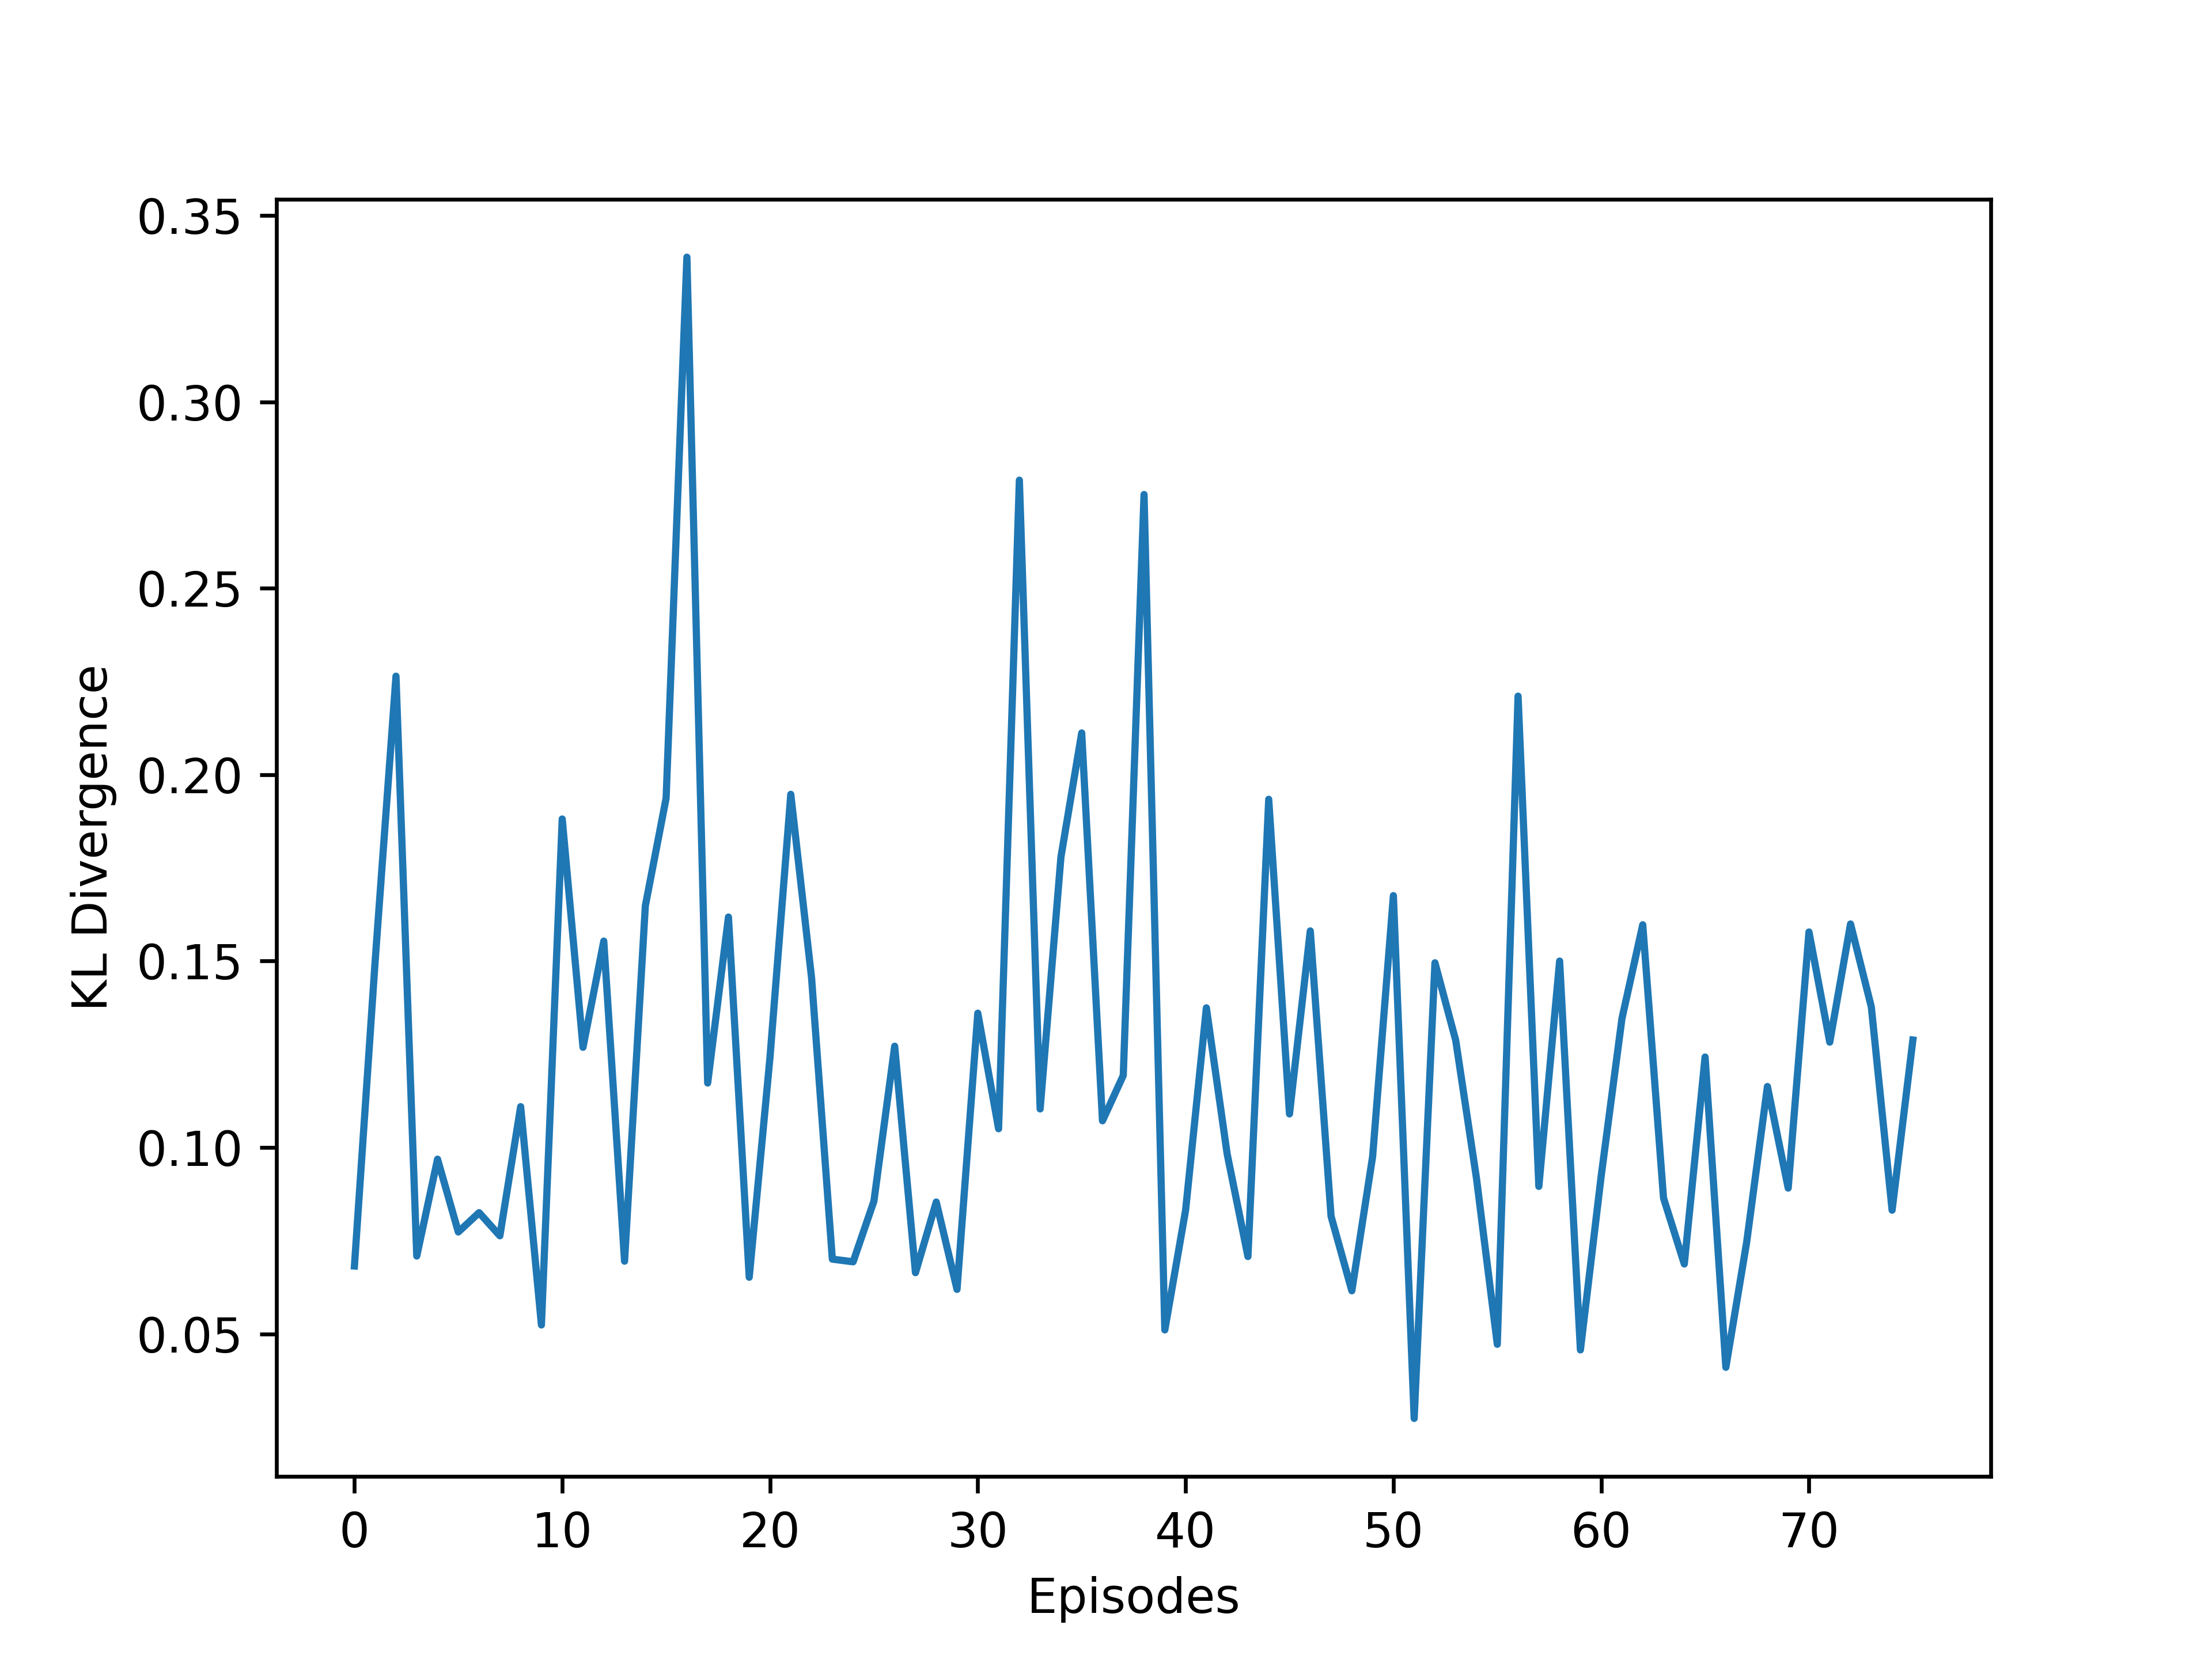
\includegraphics[width=\textwidth]{images/kld.png}
		\caption{Without agent}
		\label{fig:kld episodic style}
	\end{subfigure}
	\hfill
	\begin{subfigure}[t]{0.45\textwidth}
		\centering
		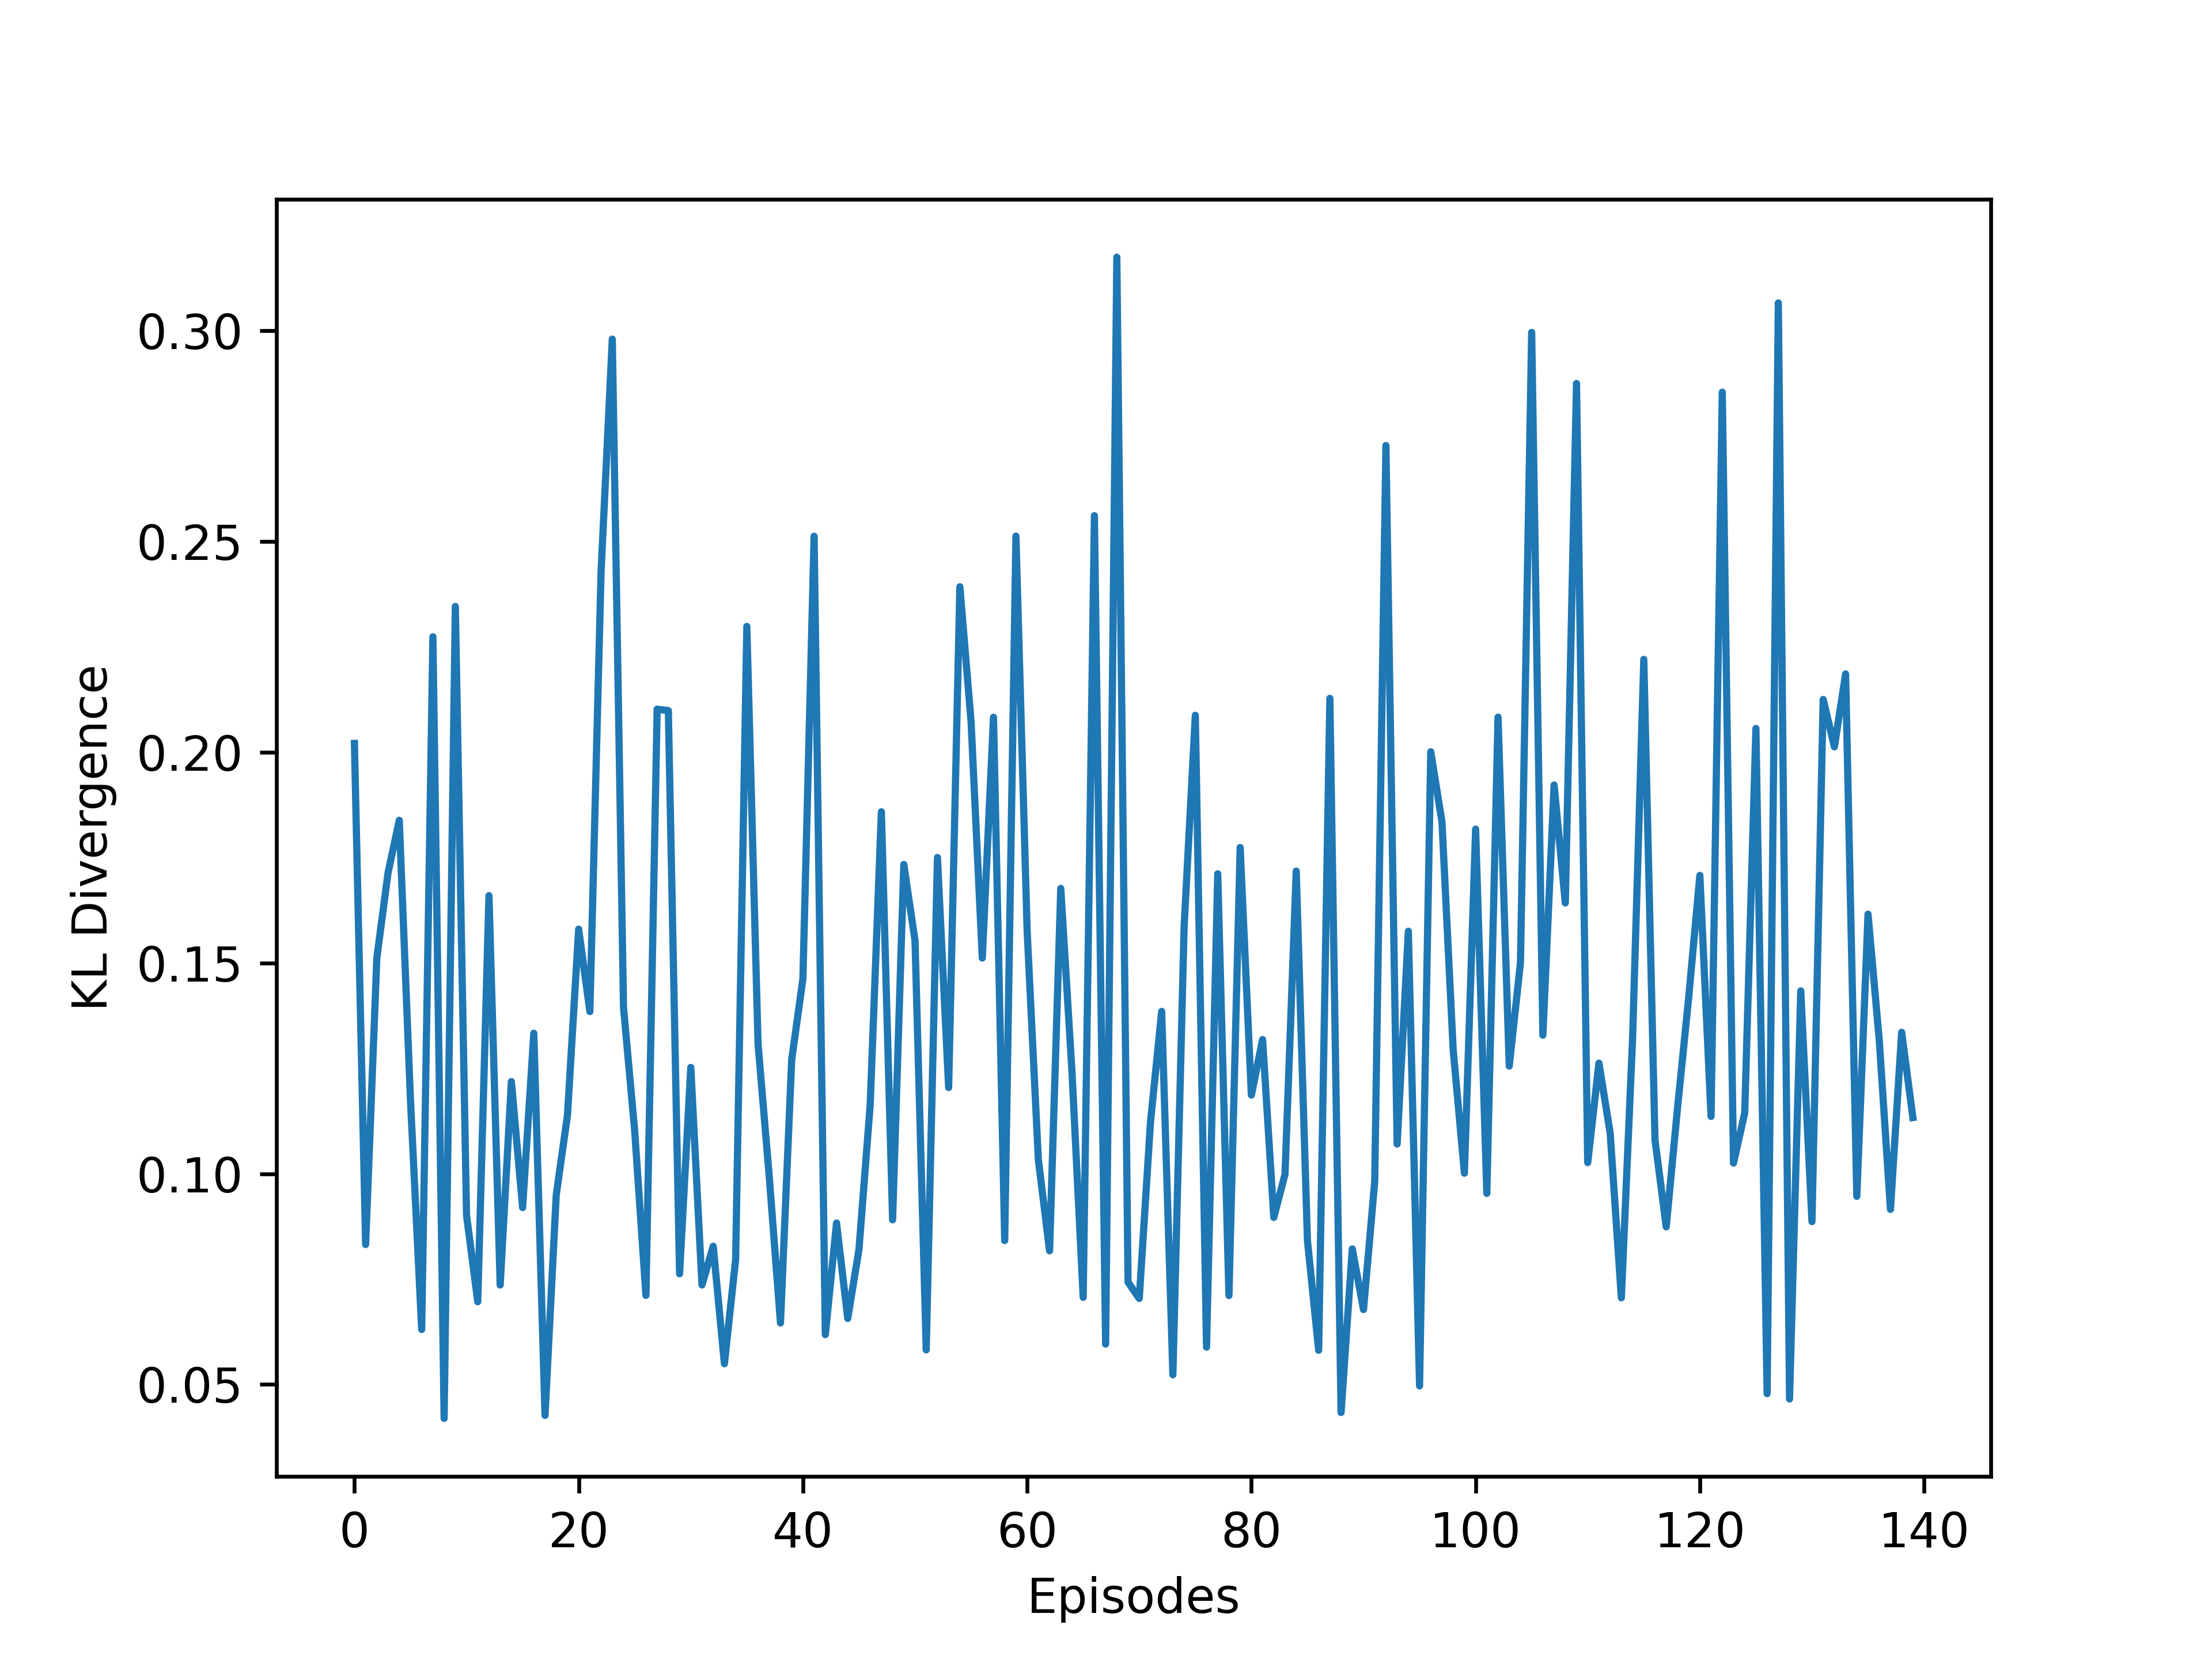
\includegraphics[width=\textwidth]{images/kld-c2.png}
		\caption{With agent}\label{fig:style deviation with agent}
	\end{subfigure}
	\caption{\label{fig:driving styles} KL divergence of episodic style from baseline.}
\end{figure}

We compute the KL-divergence of the distributions of other episodes from the baseline as an evaluation of the driving style drift. To estiamte the driving style with a sequential model is more precise but would add too much complexity to the evaluation process. Fig.\@\ref{fig:kld episodic style} shows the KL-divergence of driving style in each episode from the average, while Fig.\@\ref{fig:style deviation with agent} shows the KL-divergence for around 140 episodes with the agent while the training process goes on for a day of test drives. It can be seen that within a short time range, the KL divergence is smaller than 0.3 and the driving styles both with or without agent are stable.

\subsubsection{Results}\label{sec:results_small}

The test drives are conducted in a proving ground with a fixed vehicle, driver and route and the speed profile defined in Fig.\@\ref{fig:speed profile for traning}. With each episode of around 20 seconds, the breaks bewteen the episodes and occasional interrupts, we are able to finish around 60 consecutive episodes in 3 hours for each test run. Each run reloads the model weights and the pedal map which the last run saved and the agent is continuously updated by the training during the test run. Fig.\@\ref{fig:consumption reduction ddpg} depicts the energy consumption trends for the training of 3 weeks. Each curve corresponds to a test run.

\begin{figure}[ht]
	\centering
	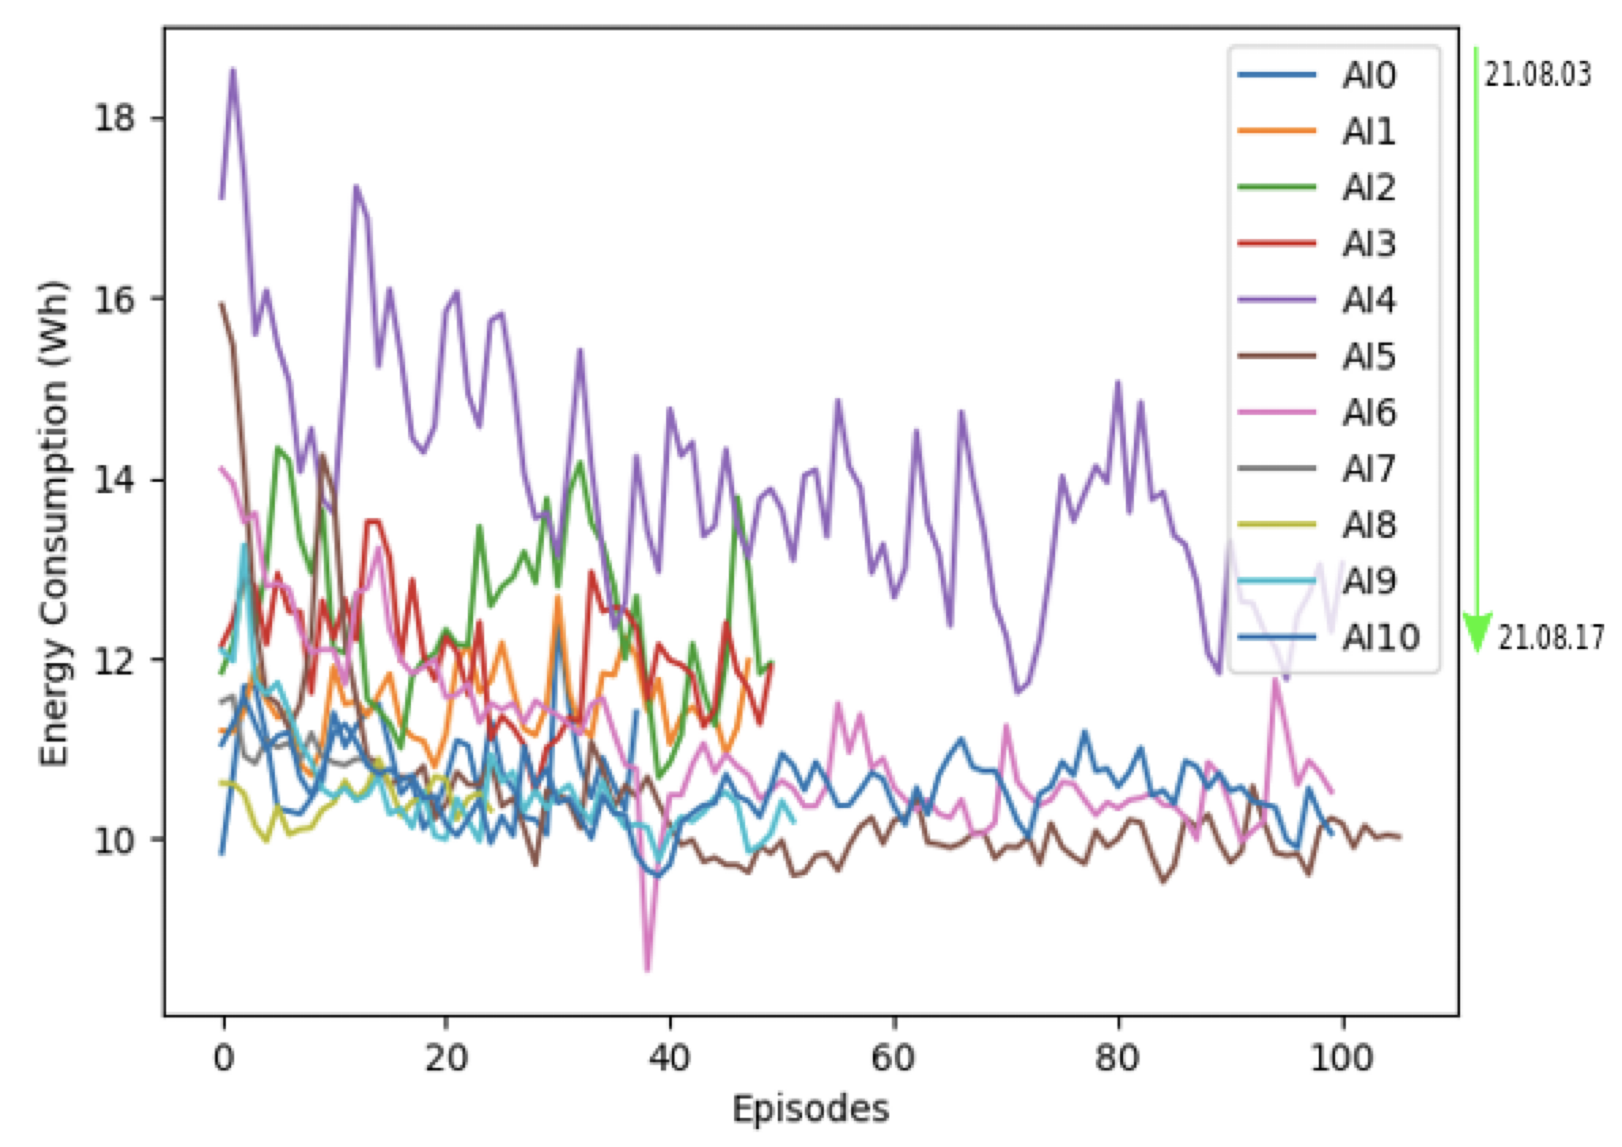
\includegraphics[width=0.6\textwidth]{images/ddpg-training1.png}
	\caption{Energy consumption reduction during training}\label{fig:consumption reduction ddpg}
\end{figure}

We can see the energy consumption is continuously reduced within each run. The trend of consumption reduction between the runs is prominent as well. During the training, the pedal map is dynamically changed by the agent. Fig.\@\ref{fig:dynamic pedal map} shows a snapshot of the map. We can see in the lower right corner of the pedal map for low speed and small pedal opening that the agent requests larger negative torque to recapture energy from momentum.

\subsection{Public road}\label{sec:public road}

The test drive is extended to open roads where the route is much longer and the scenarios are more complex with traffic lights and pedestrian which in cases makes the vehicle halt. We run baseline drives without the agent in a regular time period to evaluate the training progress, while monitoring the driving style of the human driver. In order to increase the training efficiency, We start from a frozen model trained in Sec.\@\ref{sec:training} and schedule a curriculum to add complexity incrementally to the training.

The map of the first route is shown in Fig.\@\ref{fig:1st route}. The vehicle follows the loop in the clockwise direction so that it always turns right in order not to be halted by the traffic light on the corner. When the vehicle is blocked by pedestrians, the test data is simply abandoned. Fig.\@\ref{fig:openroad a speed} shows the target speed, the upperbound, the lowerbound and the actual test speed. Comparing to the episode in Fig.\@\ref{fig:speed profile for traning}, the first route has right turns and is much longer.

\begin{figure}[htbp]
	\centering
	\begin{subfigure}[t]{0.4\textwidth}
		\centering
		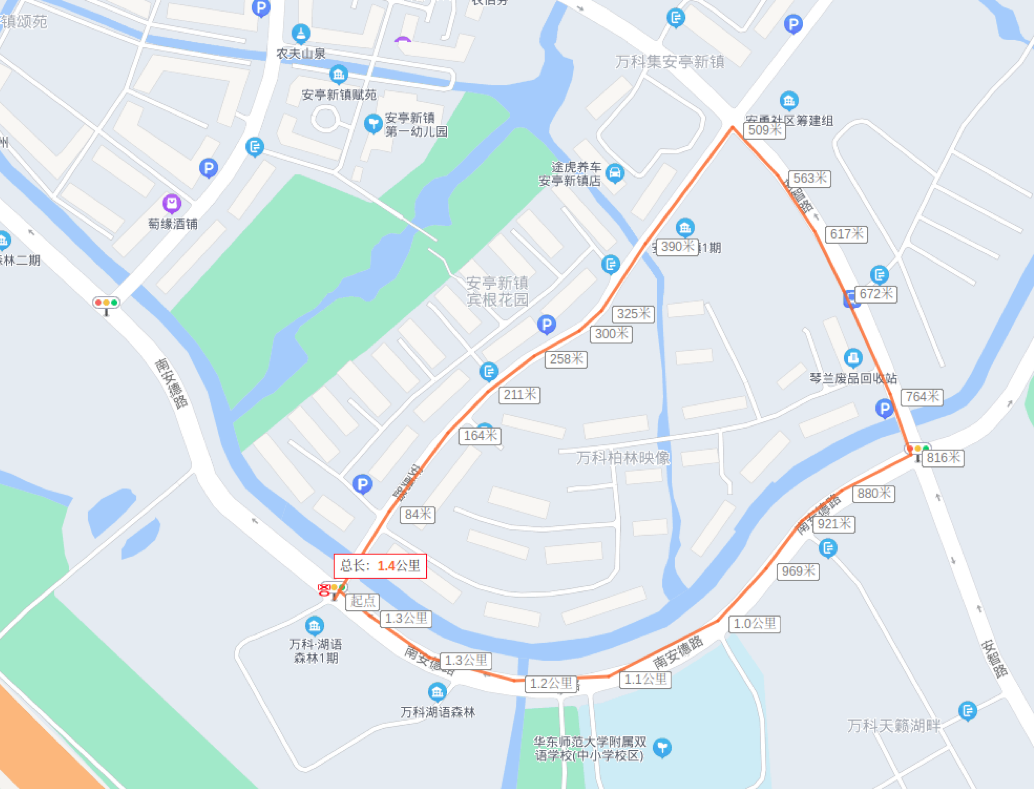
\includegraphics[width=\textwidth]{images/openroad_a_map.png}
		\caption{The 1st. route}\label{fig:1st route}
	\end{subfigure}
	\quad\quad
	\begin{subfigure}[t]{0.4\textwidth}
		\centering
		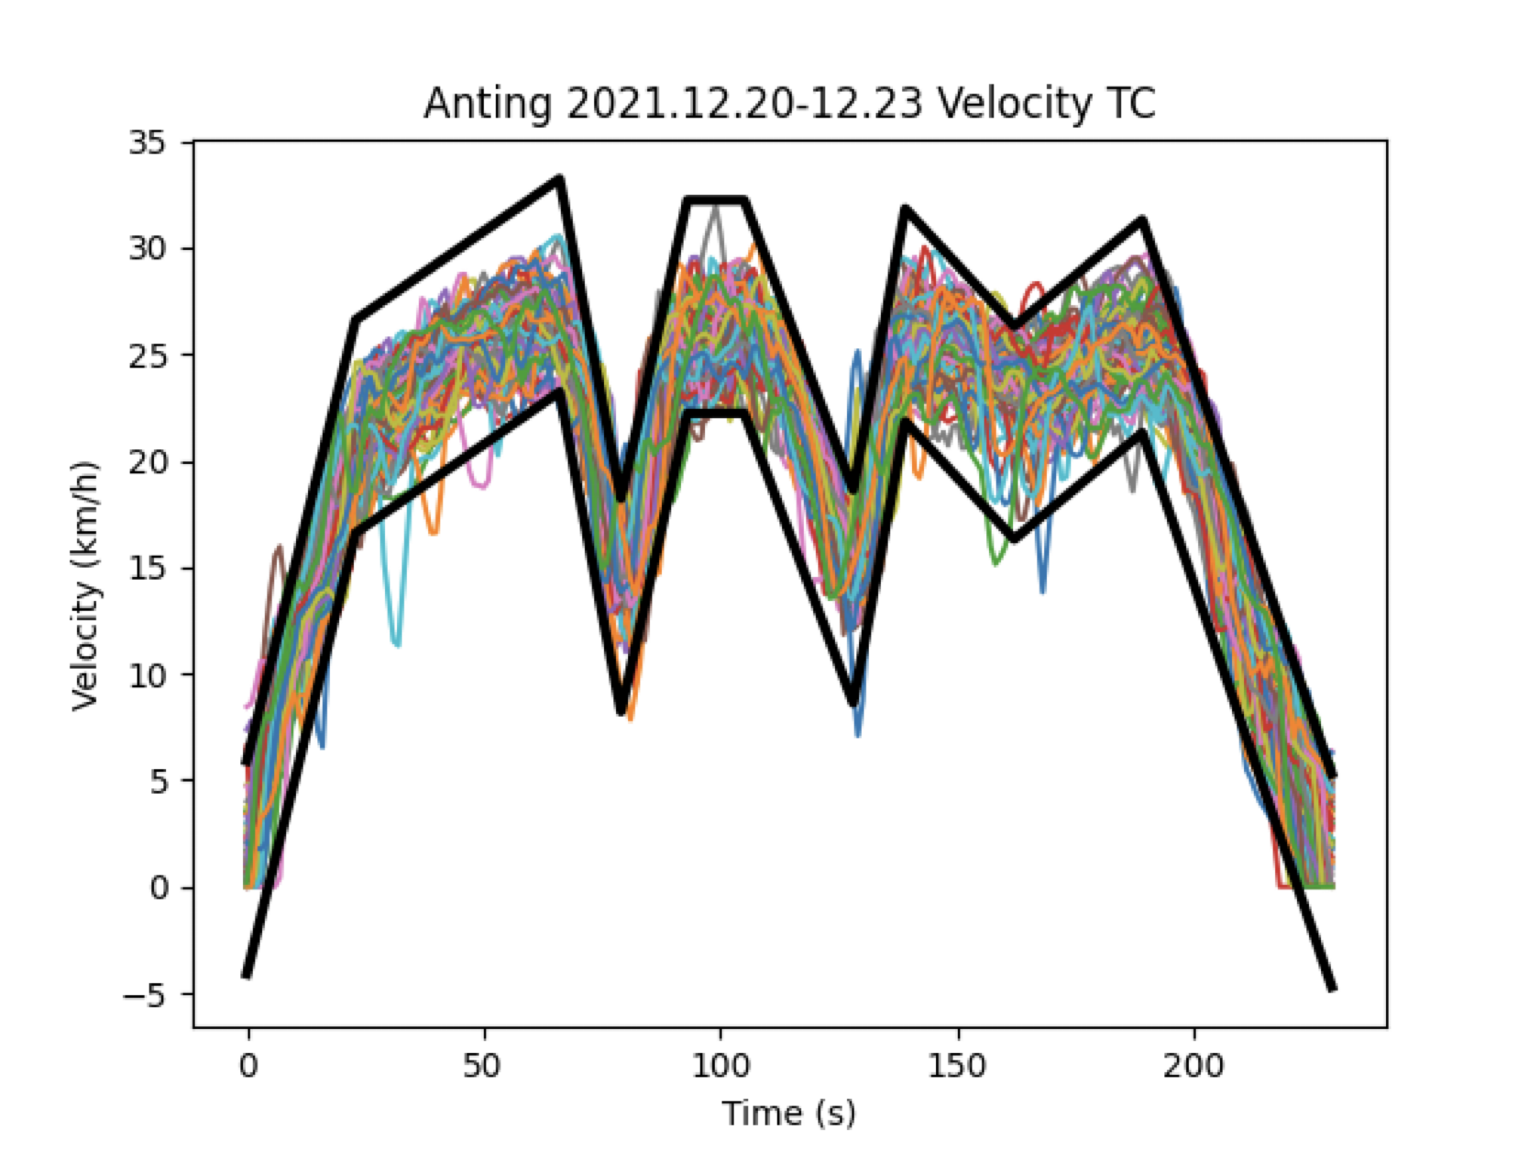
\includegraphics[width=\textwidth]{images/openroad_a_velocity.png}
		\caption{Speed of the episodes}\label{fig:openroad a speed}
	\end{subfigure}
	\caption{Test drive on the 1st. route\label{fig:open road a}}
\end{figure}

The test drive on the 1st.\@ route takes 9 days over 3 weeks and the result is depicted in Fig.\@\ref{fig:openroad a consumption}. For every week, we run baseline drives while switching off agent and compare the episodes with the agent in the same week with the baseline. The consumption reduction is shown in Tab.\@\ref{tab:openroad a result}. It should be noted that a consumption increase in week 2 is due to a temperature drop, which cause the battery management system to turn on battery heating and increase the overall consumption. This indicates that the EOSEV system is weather resistant. Comparing to each baselines, the average consumption reduction is $7\%\sim8\%$.

In Fig.\@\ref{fig:openroad a style}, the orange and the blue curve correspond to the KL divergence of the episodic driving style with and without the agent respectively. A drift in driving style while training can be seen over around 600 episodes. In the long run, the driving style will be impacted by the agent changing the powertrain behavior, if the driver is exploring a cooperative driving strategy. The agent is adaptive to this change.

\begin{figure}[hbtp]
	\begin{minipage}[b]{0.3\linewidth}
		\centering
		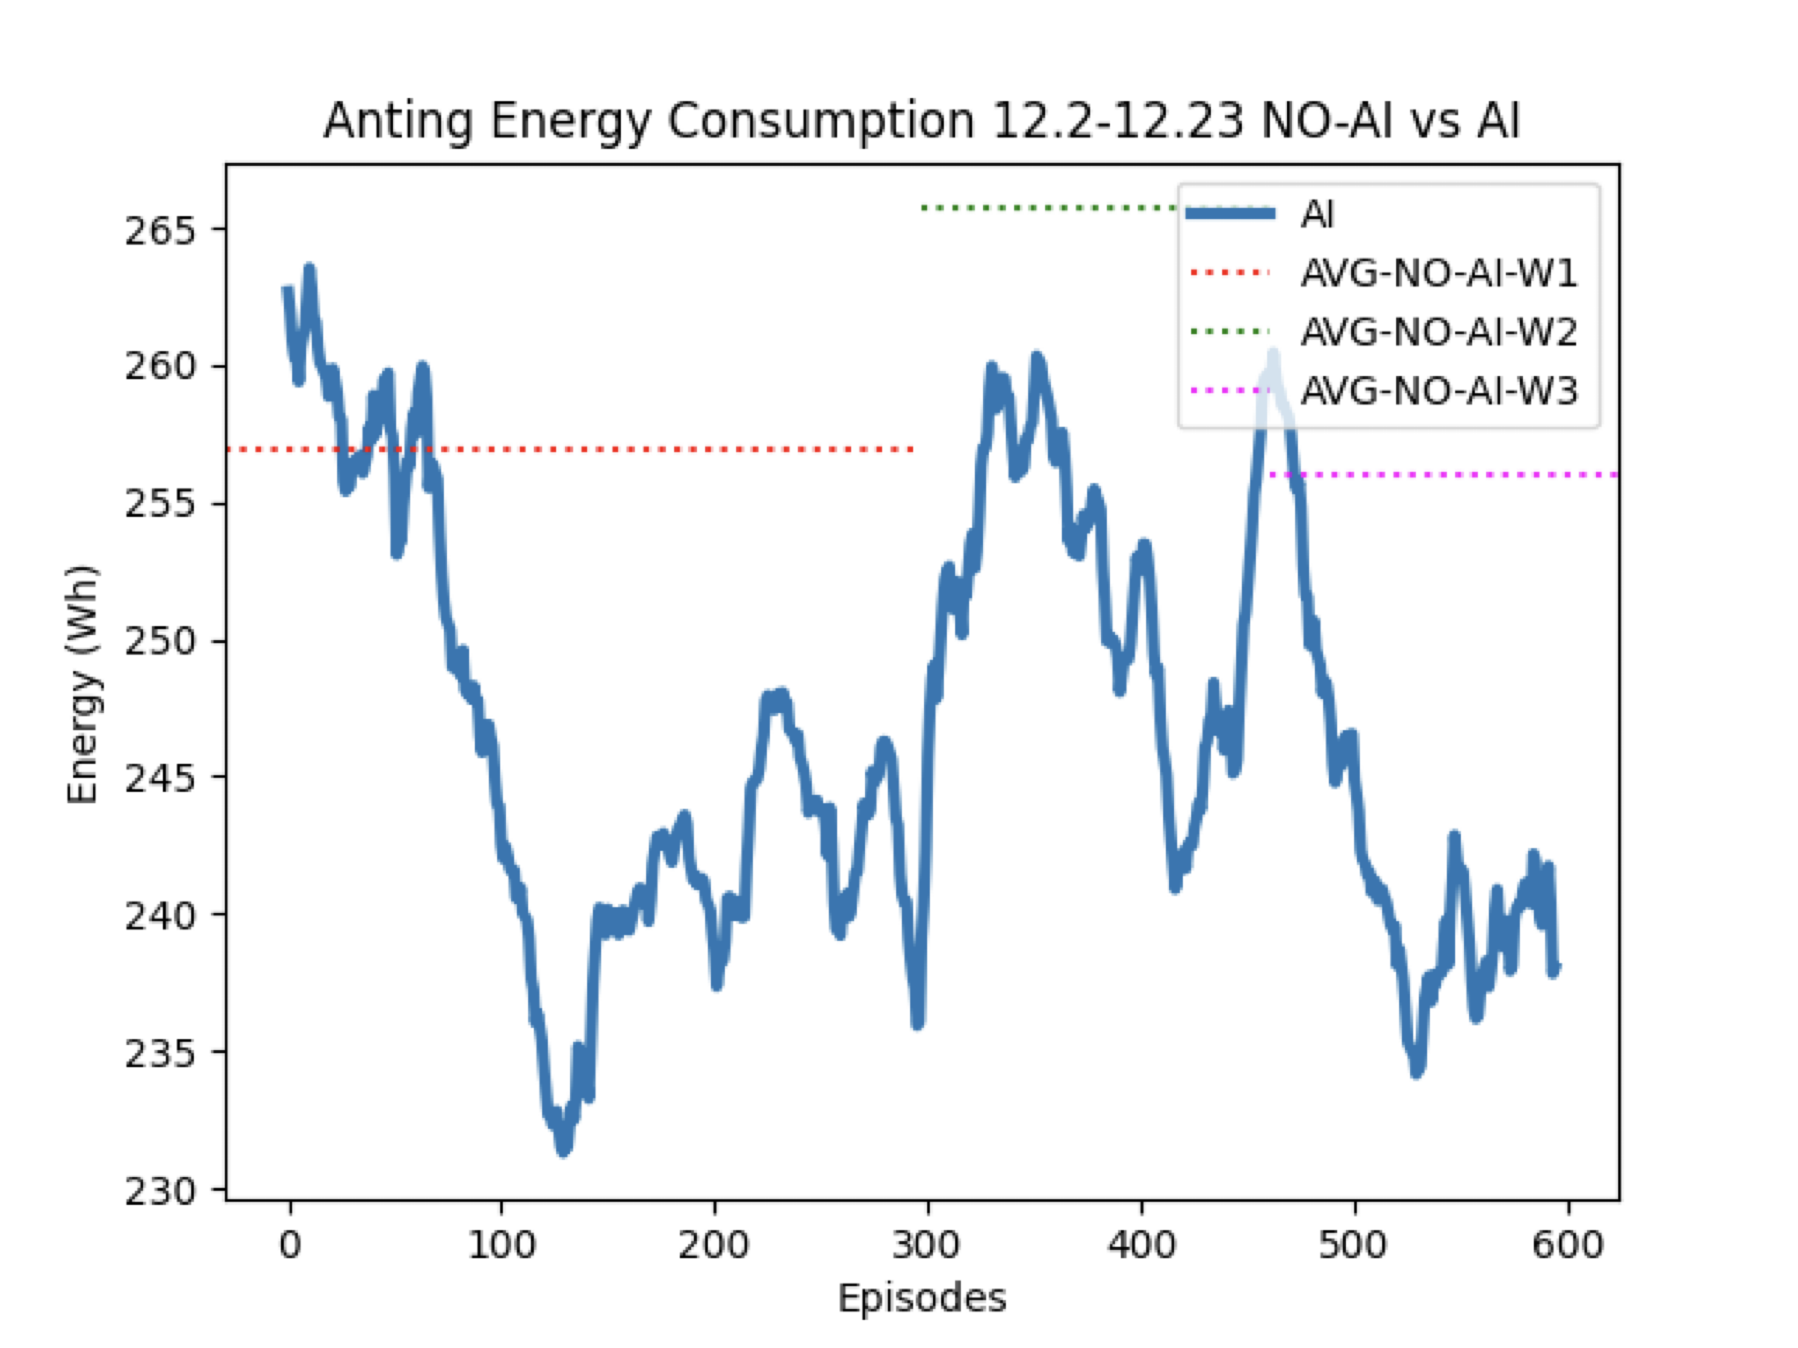
\includegraphics[width=\textwidth]{images/openroad_a_consumption.png}
		\caption{Energy consumption}\label{fig:openroad a consumption}
	\end{minipage}
	\hfill
	\begin{minipage}[b]{0.3\linewidth}
		\centering
		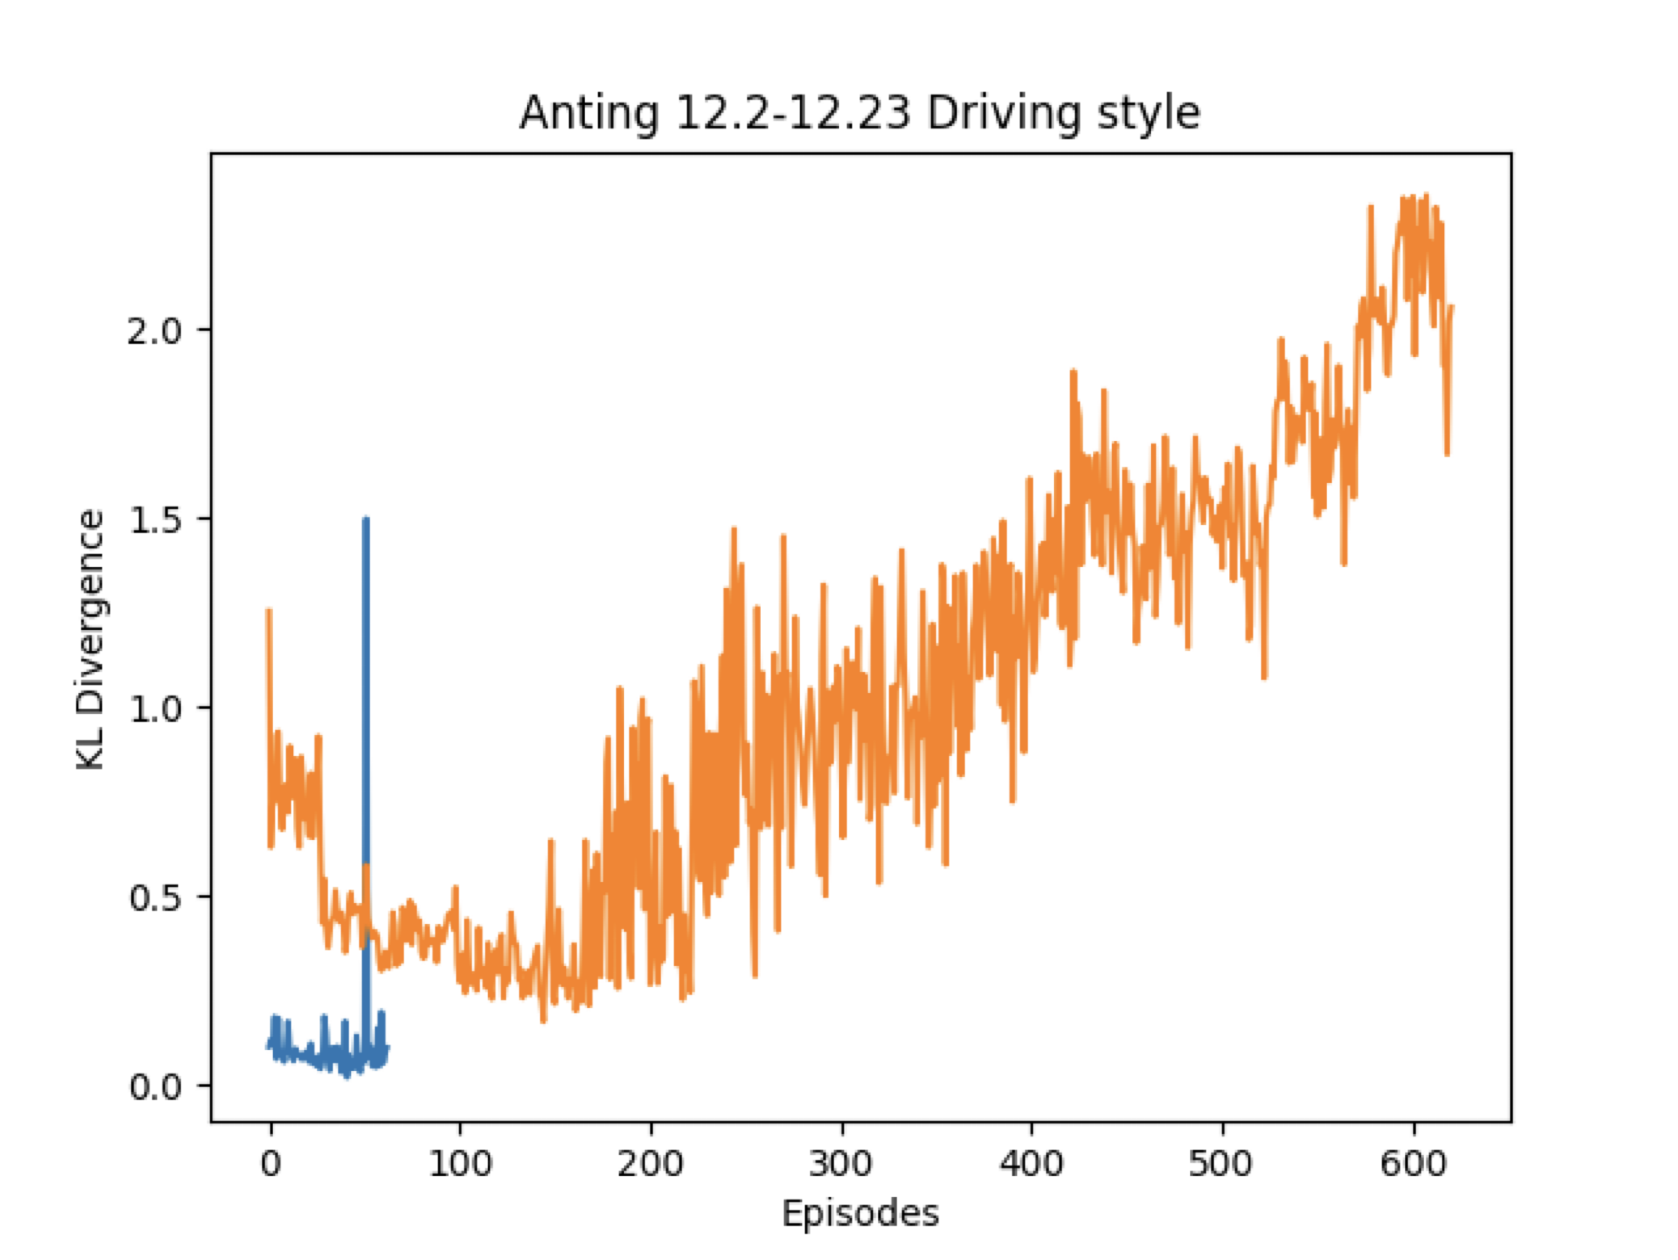
\includegraphics[width=\textwidth]{images/openroad_a_style.png}
		\caption{Driving style drift}\label{fig:openroad a style}
	\end{minipage}
	\hfill
	\begin{minipage}[b]{0.3\linewidth}
		\centering
		\begin{tabular}{c c c c}
			\toprule
			     & Week 1 & Week 2 & Week 3 \\
			\midrule
			base & 256.9  & 265.7  & 256.0  \\
			Agt. & 245.0  & 251.9  & 243.7  \\
			Red. & 8.16\% & 7.56\% & 7.03\% \\
			\bottomrule
		\end{tabular}
		\captionof{table}{\label{tab:openroad a result}Results of training on the first route}
	\end{minipage}\hfill
\end{figure}

%\begin{figure}[htbp]
%	\centering
%	\begin{subfigure}[t]{0.45\textwidth}
%		\centering
%		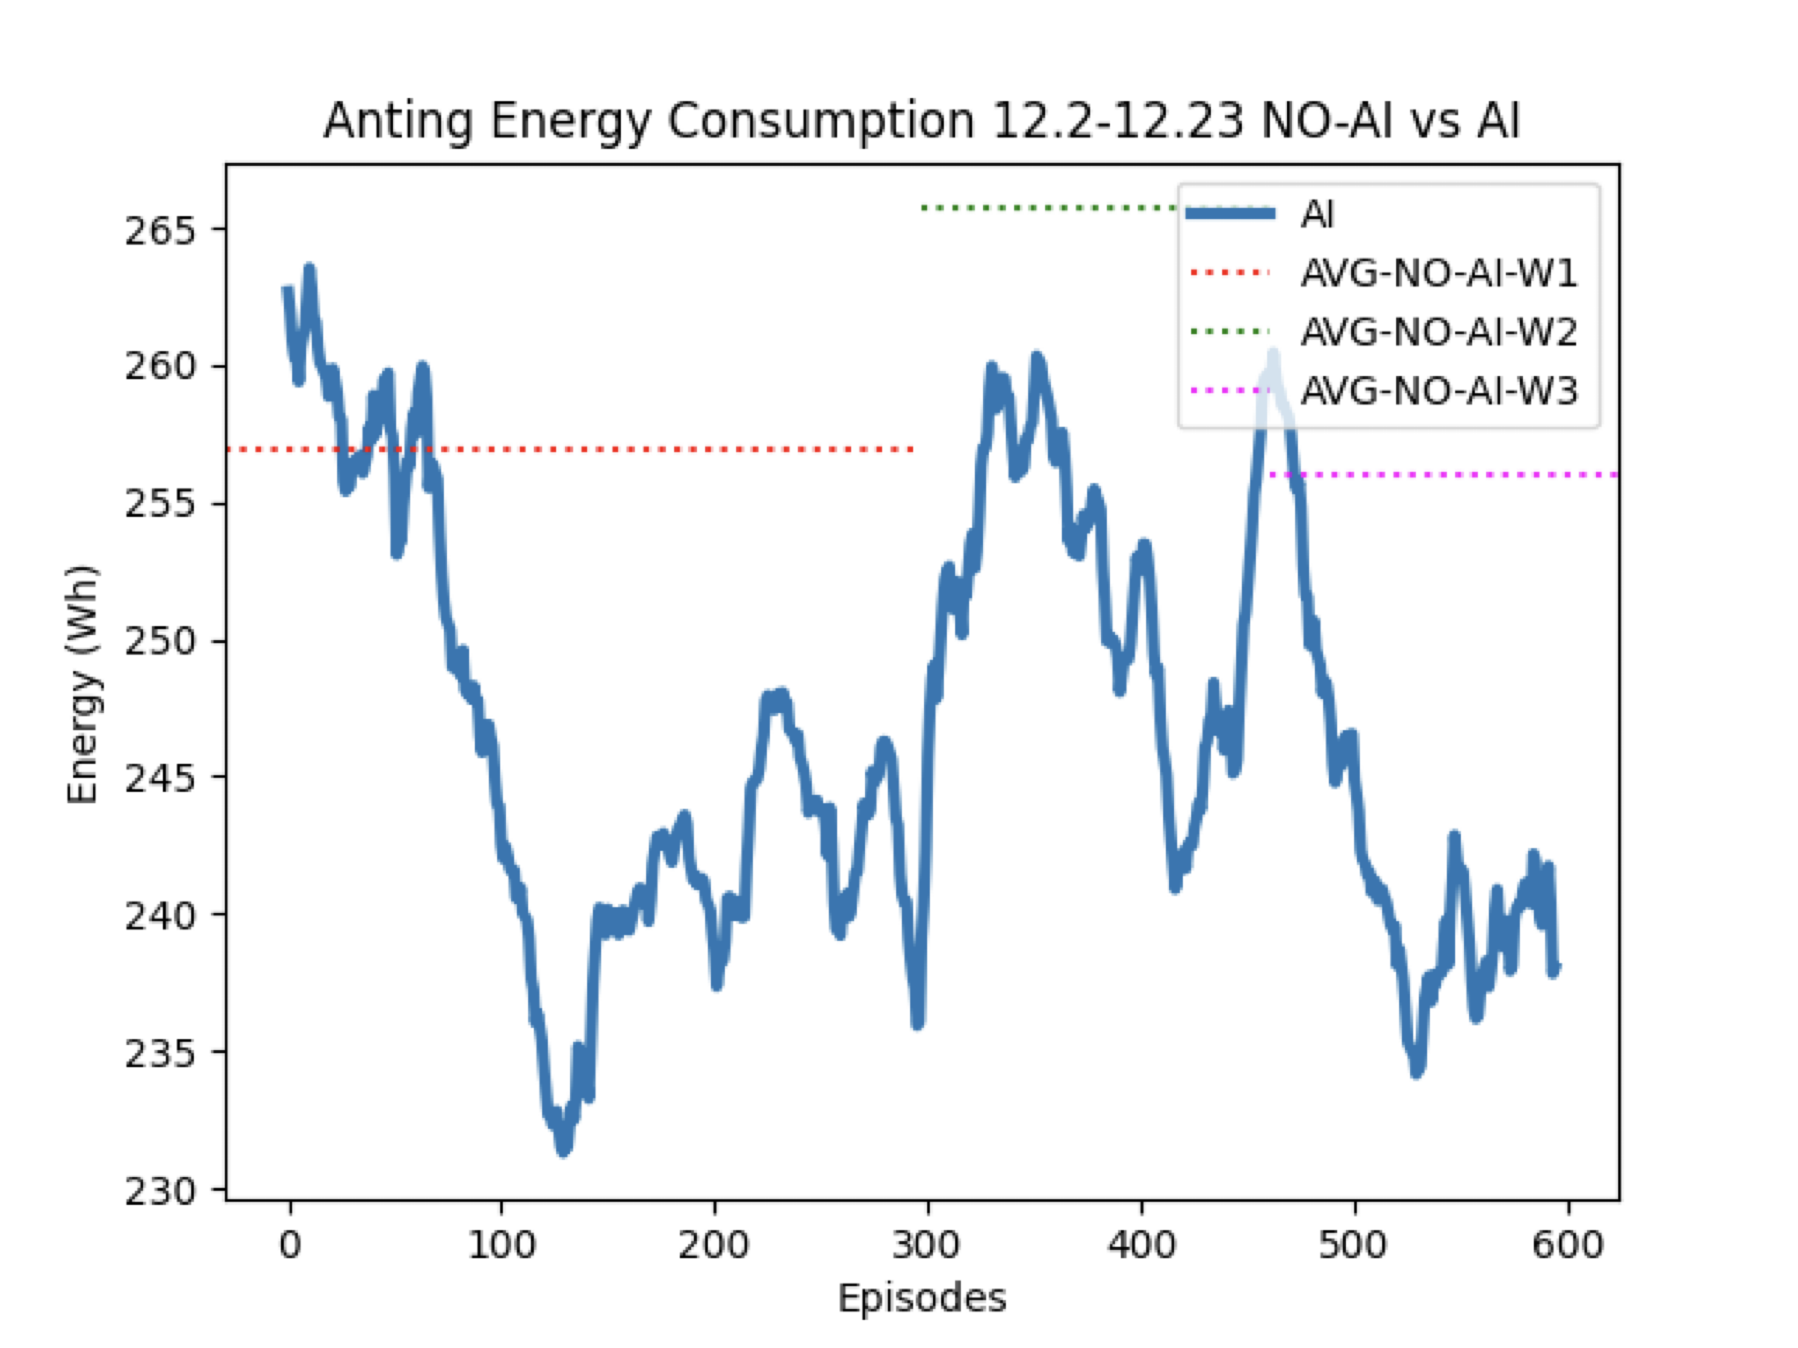
\includegraphics[width=\textwidth]{images/openroad_a_consumption.png}
%		\caption{Energy consumption}\label{fig:openroad a consumption}
%	\end{subfigure}
%	\hfill
%	\begin{subfigure}[t]{0.45\textwidth}
%		\centering
%		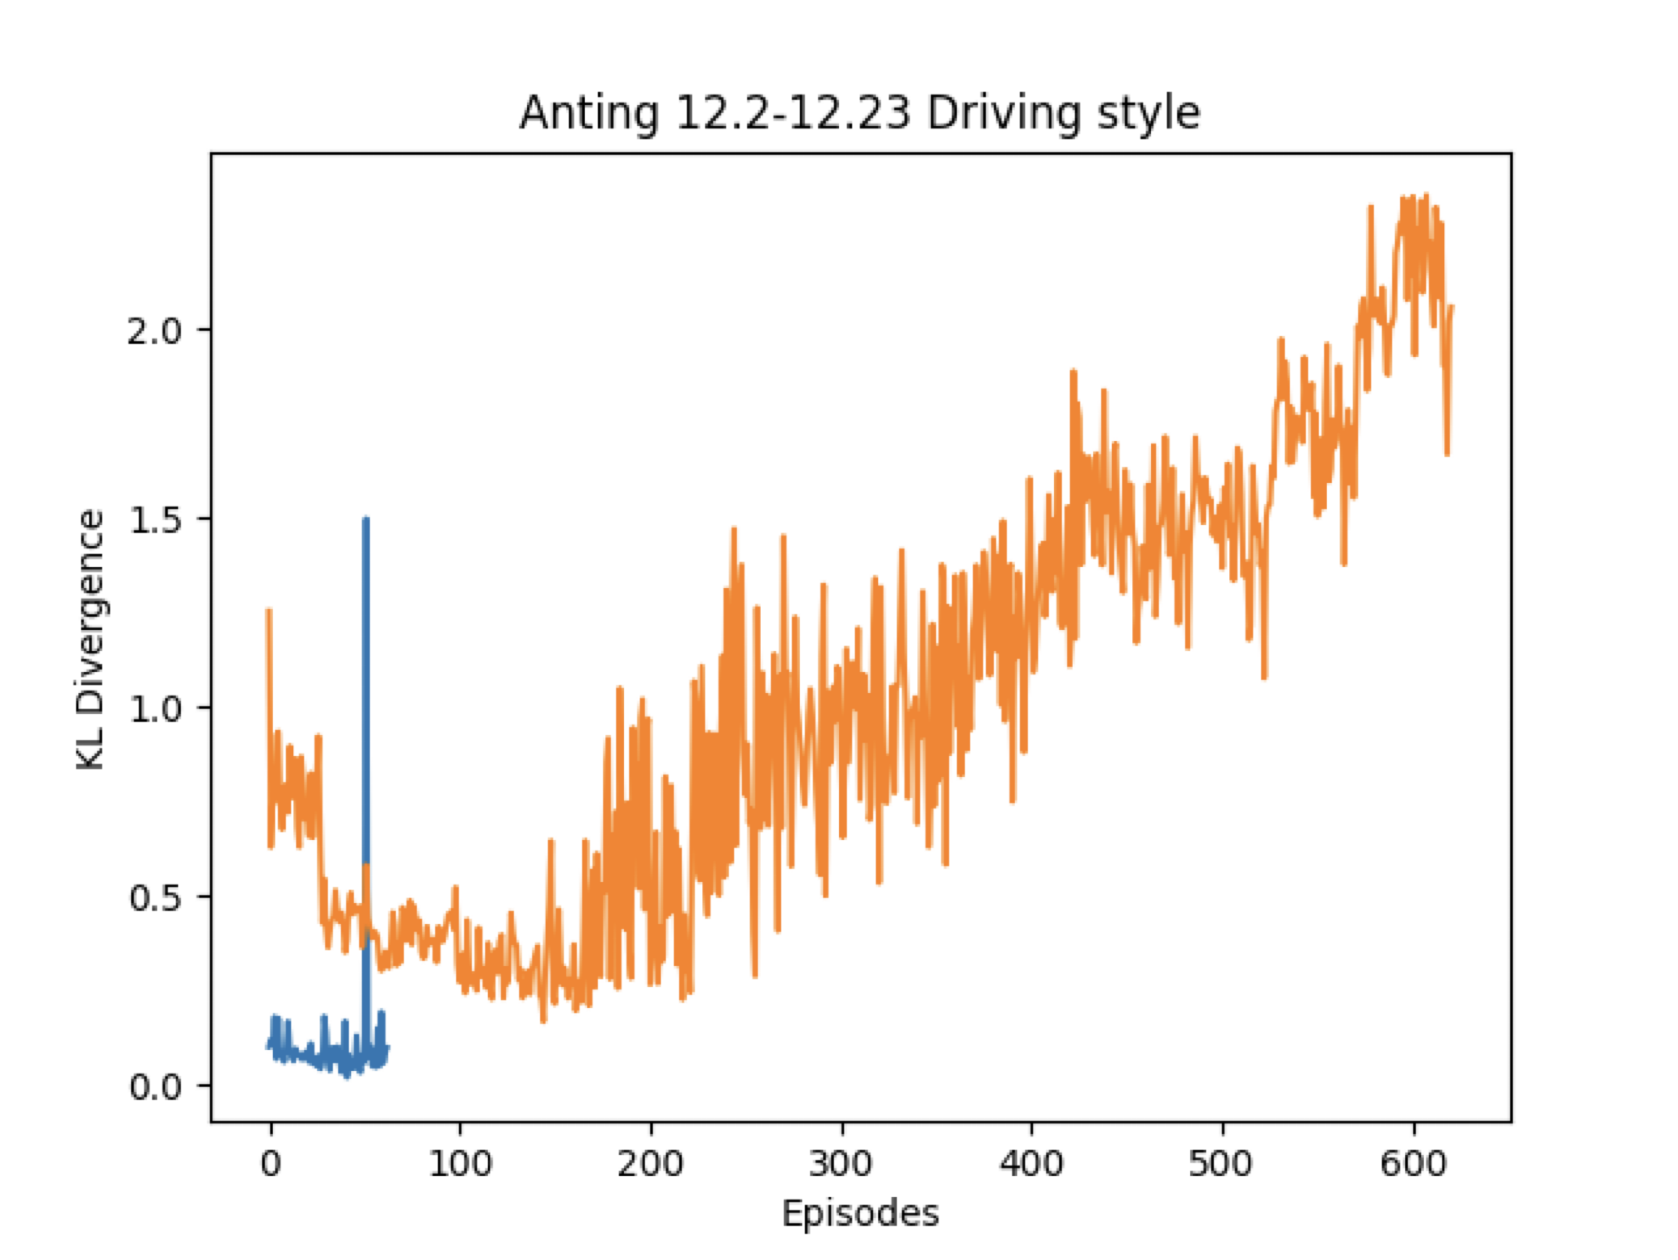
\includegraphics[width=\textwidth]{images/openroad_a_style.png}
%		\caption{Driving style drift}\label{fig:openroad a style}
%	\end{subfigure}
%	\caption{Test drive on public road\label{fig:open road a}}
%\end{figure}


\subsubsection{Transferability}\label{sec:transferable}

In order to verify the transferablility, the frozen model trained from the 1st.\@ route is used on the second route in Fig.\@\ref{fig:2nd route}, which has a different target speed profile Fig.\@\ref{fig:openroad b speed}. The result is shown in Fig.\@\ref{fig:openroad b result}. Comparing to the baseline, the consumption reduction with the frozen model without any specific fine-tuning is around 4\%. This indicates an application with a generic pre-training on typical driving scenarios and the deployment of a frozen model on the real roads without training, which will simplify the production architecture and deployment cost drastically at the expense of less performance and adaptability.

\begin{figure}[htbp]
	\centering
	\begin{subfigure}[t]{0.45\textwidth}
		\centering
		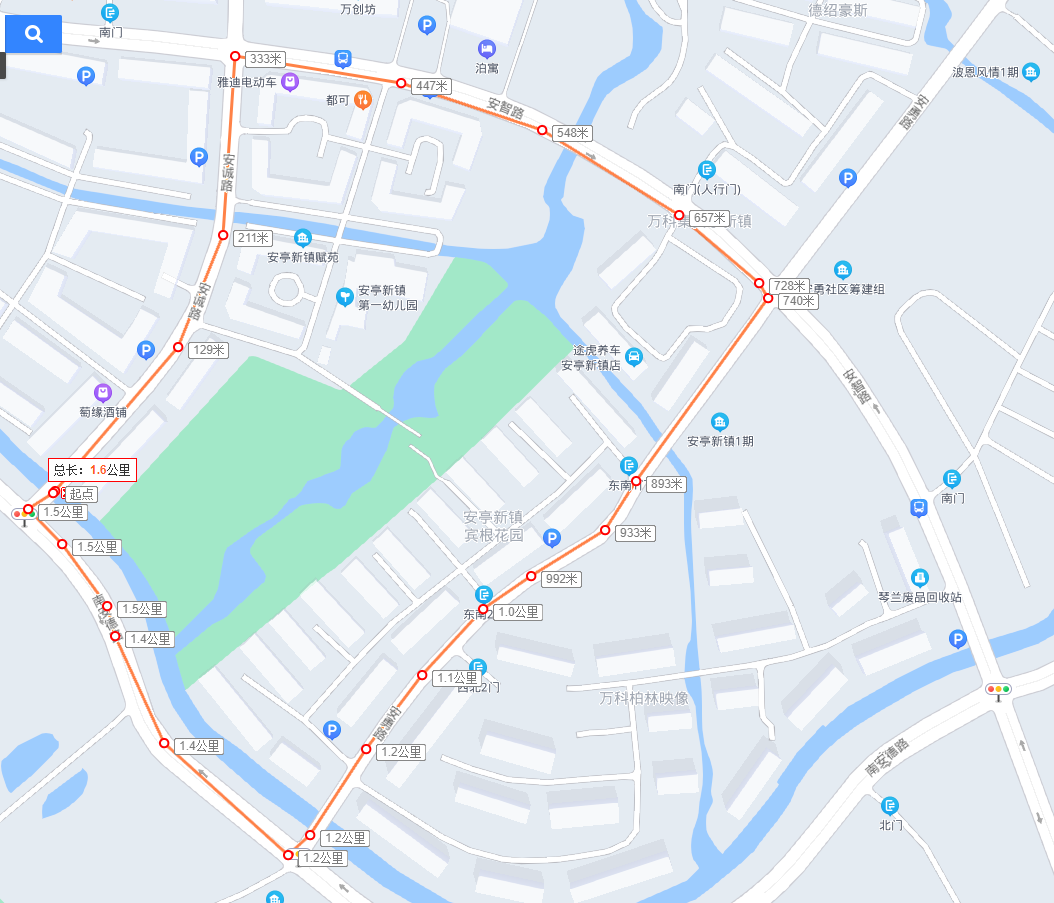
\includegraphics[width=\textwidth]{images/openroad_b_map.png}
		\caption{The 2nd. Route}\label{fig:2nd route}
	\end{subfigure}
	\hfill
	\begin{subfigure}[t]{0.45\textwidth}
		\centering
		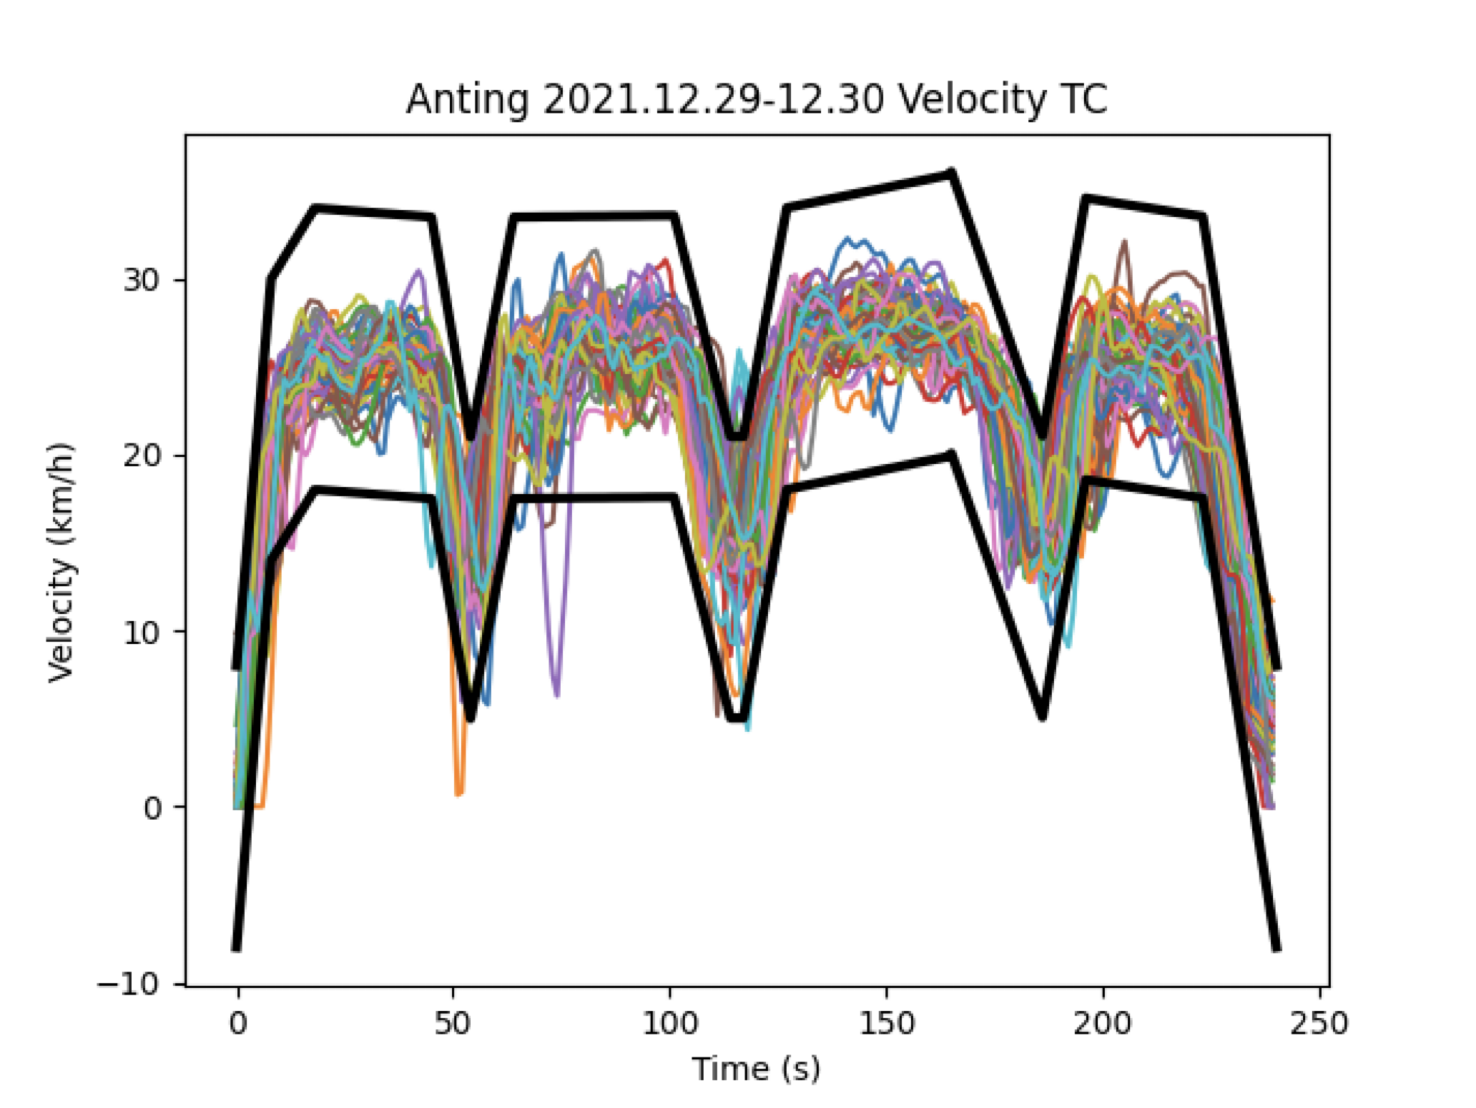
\includegraphics[width=\textwidth]{images/openroad_b_velocity.png}
		\caption{Speed of the episodes}\label{fig:openroad b speed}
	\end{subfigure}
	\caption{Test drive on the 2nd. route\label{fig:open road b}}
\end{figure}

In Fig.\@\ref{fig:openroad b style} we can see the KL divergence is smaller than 0.16 and the driving style is not drifting since the agent is frozen.

\begin{figure}[htbp]
	\centering
	\begin{subfigure}[t]{0.4\textwidth}
		\centering
		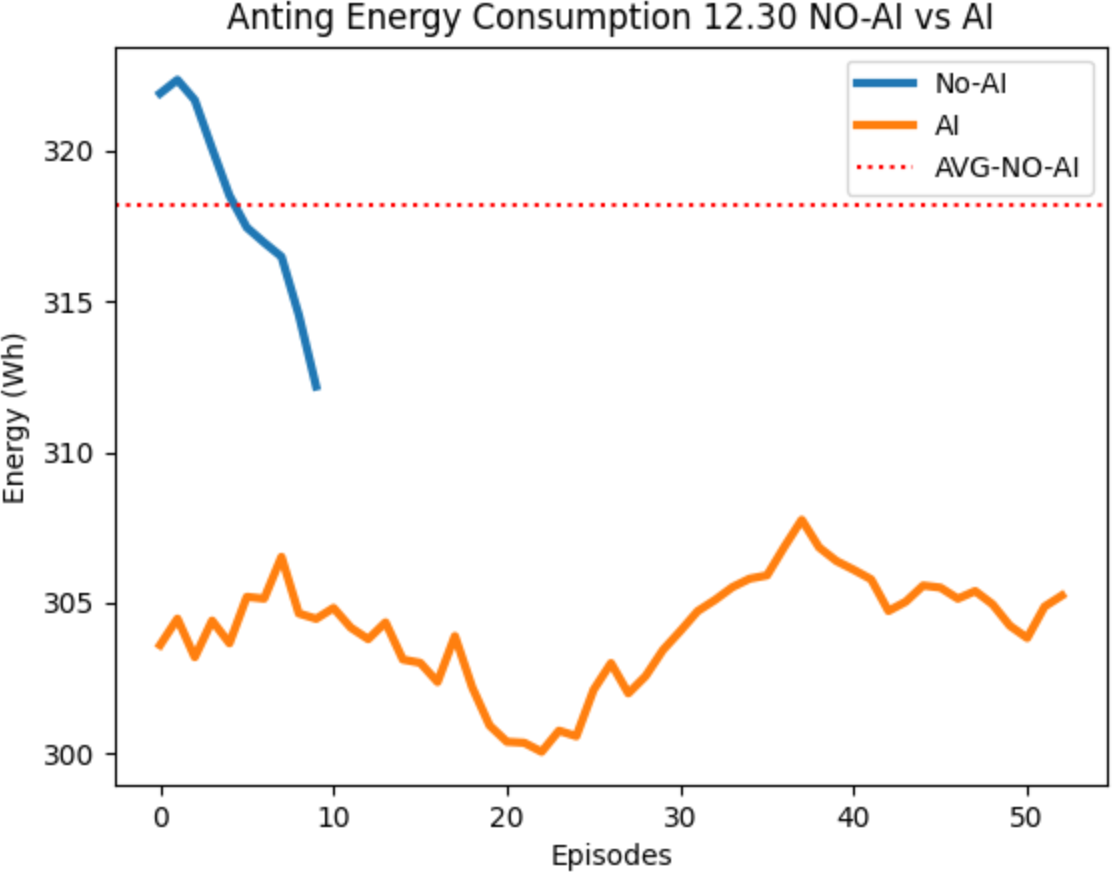
\includegraphics[width=\textwidth]{images/openroad_b_consumption.png}
		\caption{Energy consumption. The redcution is around 4\%}\label{fig:openroad b consumption}
	\end{subfigure}
	\hfill
	\begin{subfigure}[t]{0.4\textwidth}
		\centering
		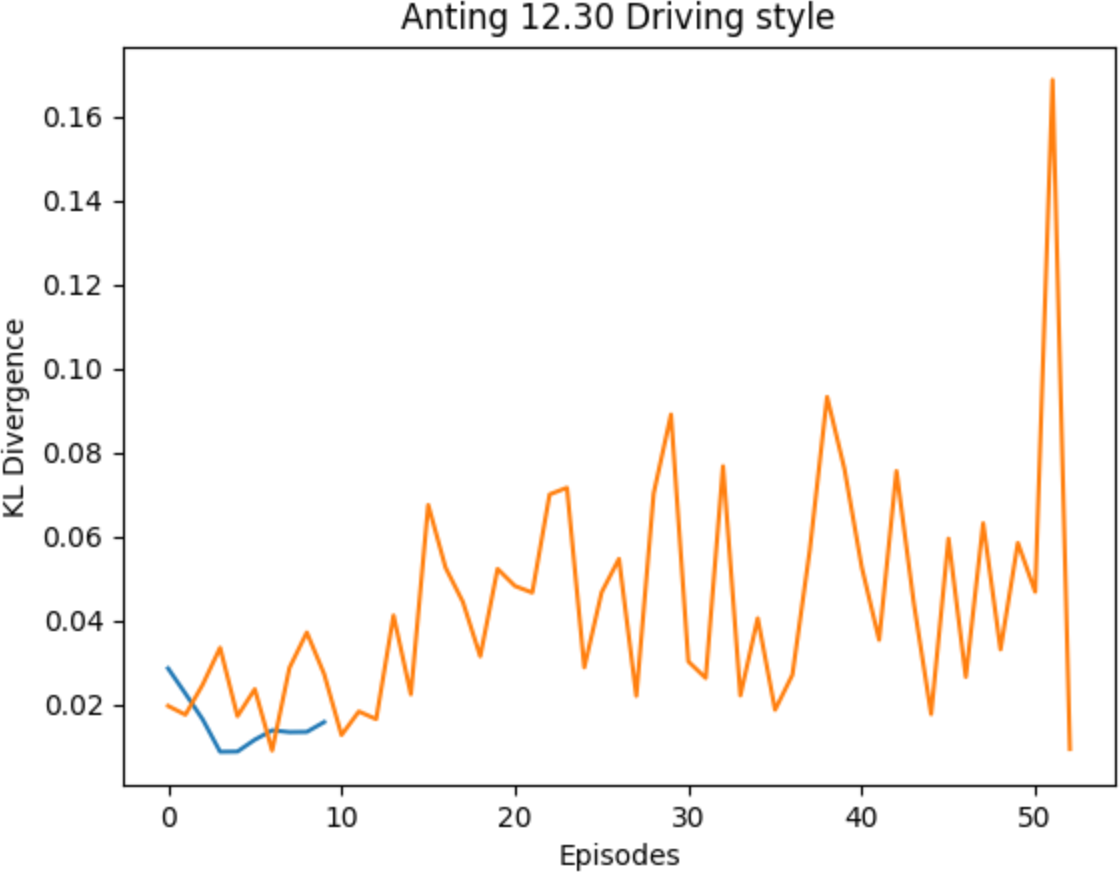
\includegraphics[width=\textwidth]{images/openroad_b_style.png}
		\caption{Driving style drift}\label{fig:openroad b style}
	\end{subfigure}
	\caption{Result on the second route\label{fig:openroad b result}}
\end{figure}

\subsubsection{Multimodality}\label{sec:multimodal}

The agent should have multimodal policies to handle different scenarios. Without multimodal capability, multimodal data will mean noise to the agent, so that it will not learn the correct strategies for different data modes.  However, neural networks can approximate multimodal functions very well. It's important to verify that the agent can deal with complex multimodal scenarios efficiently.

In order to test the multimodality, we test on the first route but treat halting scenarios due to traffic lights or pedestrians as valid. In test drives we ask the driver to tag the observations of the halting or non-halting state at every right turn for later analysis. Since we have three right turns, this corresponds to 8 modes of data depending states on the right turns to be halted or not. We test for a long time so as to get sufficient sample episodes for each mode. In the analysis, we filter out the different modes for comparison. For each mode, we define the target speed profile, calculate the baseline and the episodic consumption. For the sake of brevity, we only show two modes in Fig.\@\ref{fig:open road mm 000} for not halting at all turns and Fig.\@\ref{fig:open road mm 111} for halting at all turns.

\begin{figure}[htbp]
	\centering
	\begin{subfigure}[t]{0.3\textwidth}
		\centering
		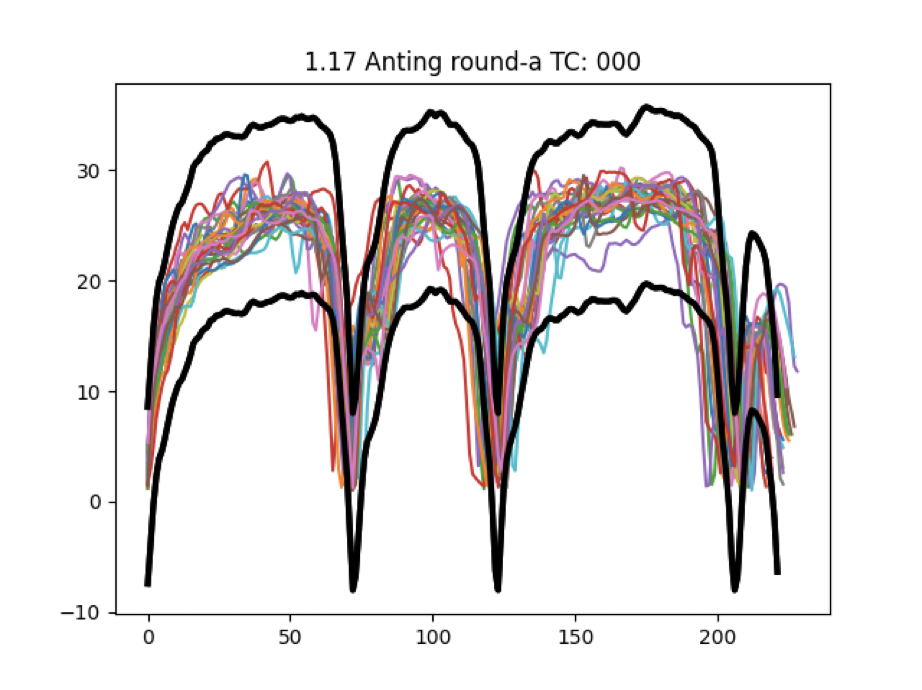
\includegraphics[width=\textwidth]{images/openroad_mm_000_velocity.png}
		\caption{Target speed profile and the test speed}\label{fig:openroad mm 000 velocity}
	\end{subfigure}
	\hfill
	\begin{subfigure}[t]{0.3\textwidth}
		\centering
		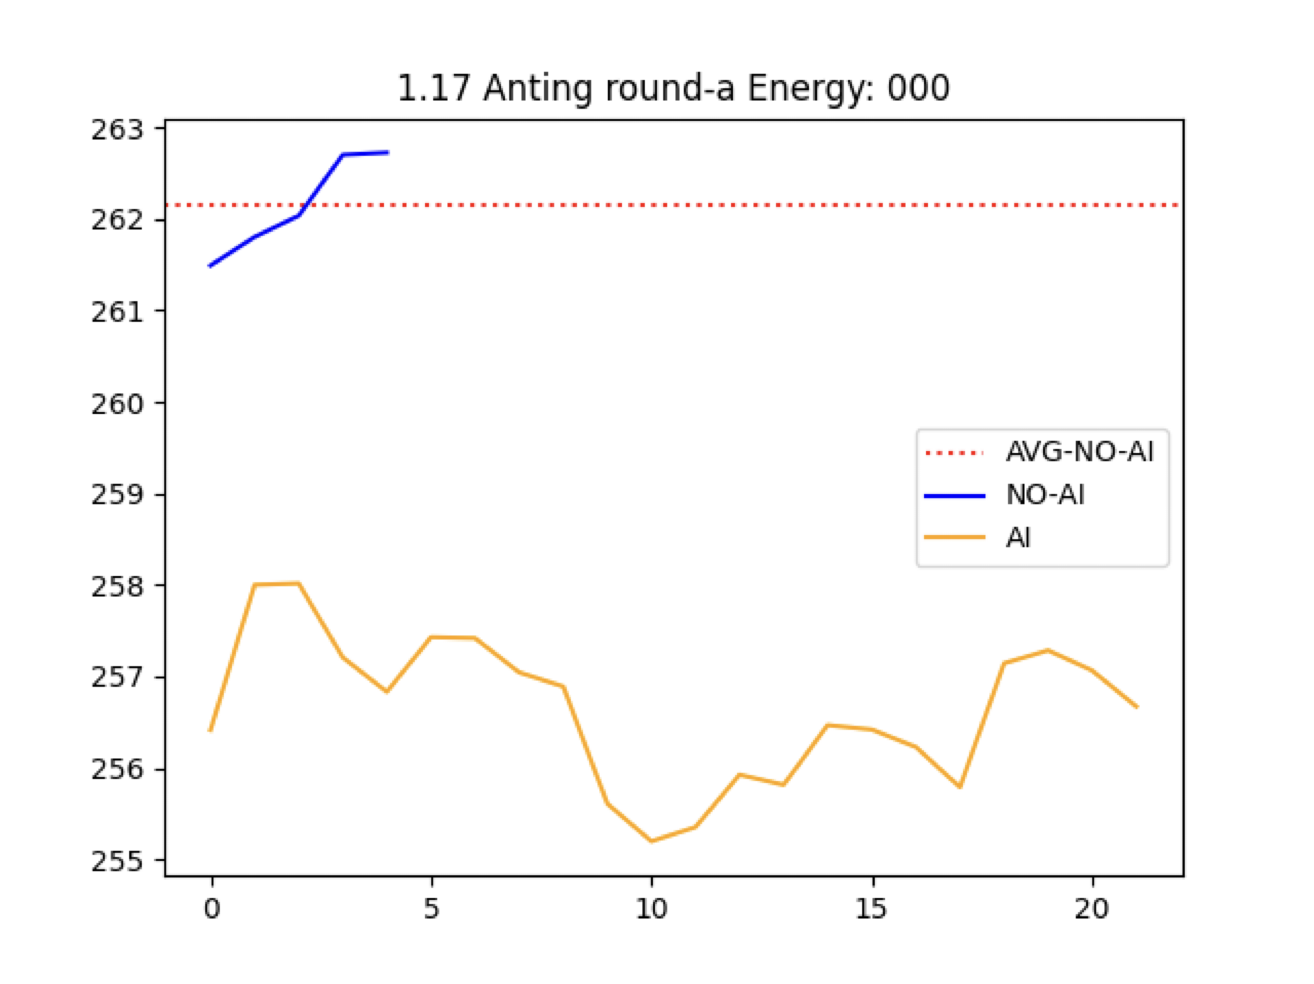
\includegraphics[width=\textwidth]{images/openroad_mm_000_consumption.png}
		\caption{Energy consumption. The reduction is 9.5\% in average.}\label{fig:openroad mm 000 consumption}
	\end{subfigure}
	\hfill
	\begin{subfigure}[t]{0.3\textwidth}
		\centering
		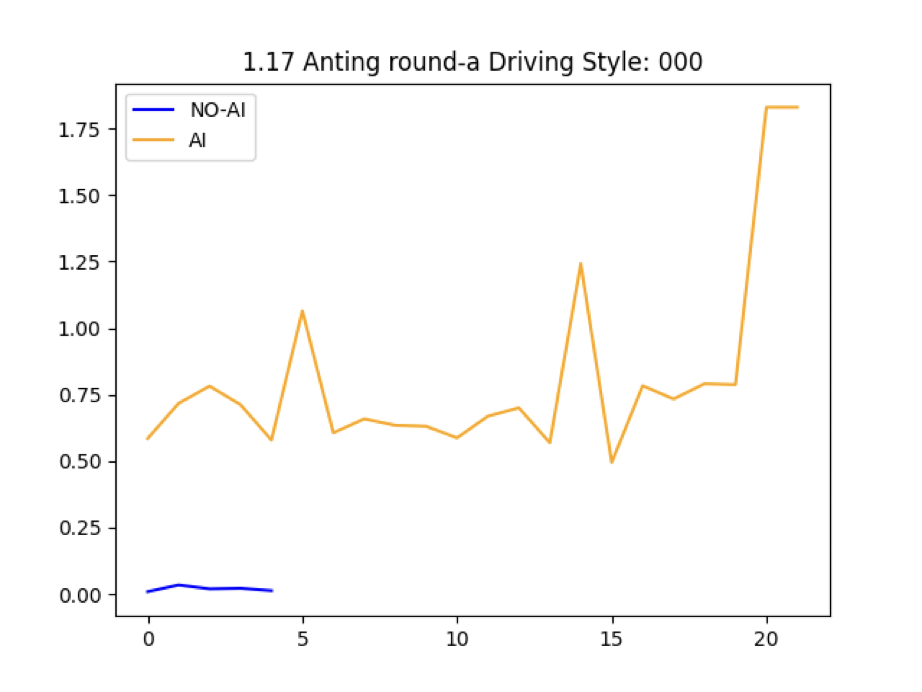
\includegraphics[width=\textwidth]{images/openroad_mm_000_style.png}
		\caption{Driving style drift}\label{fig:openroad mm 000 style}
	\end{subfigure}
	\caption{Scenarios for not halting at all turns\label{fig:open road mm 000}}
\end{figure}


\begin{figure}[htbp]
	\centering
	\begin{subfigure}[t]{0.3\textwidth}
		\centering
		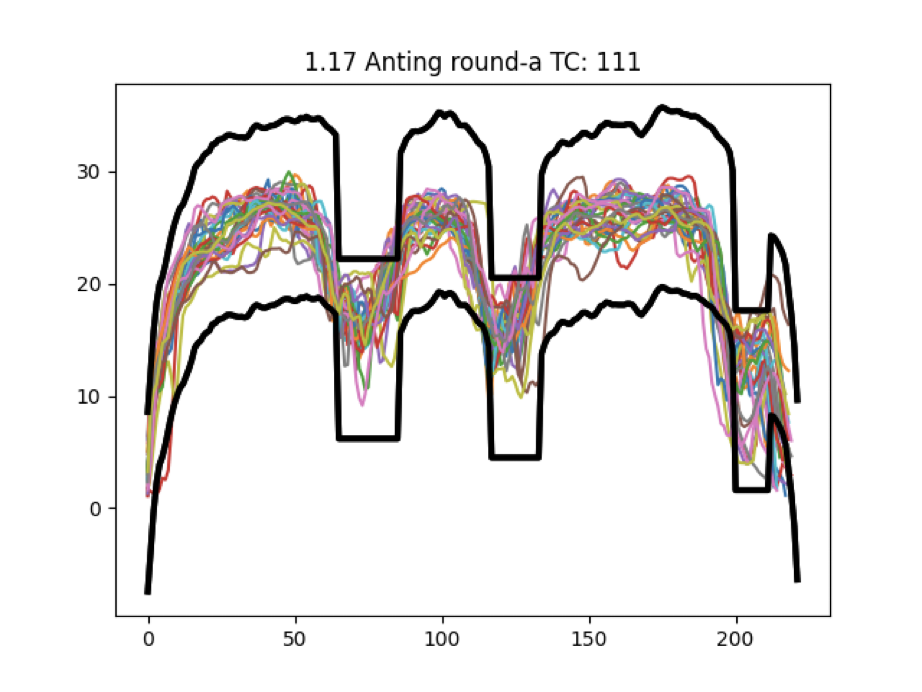
\includegraphics[width=\textwidth]{images/openroad_mm_111_velocity.png}
		\caption{Target speed profile and the test speed}\label{fig:openroad mm 111 velocity}
	\end{subfigure}
	\hfill
	\begin{subfigure}[t]{0.3\textwidth}
		\centering
		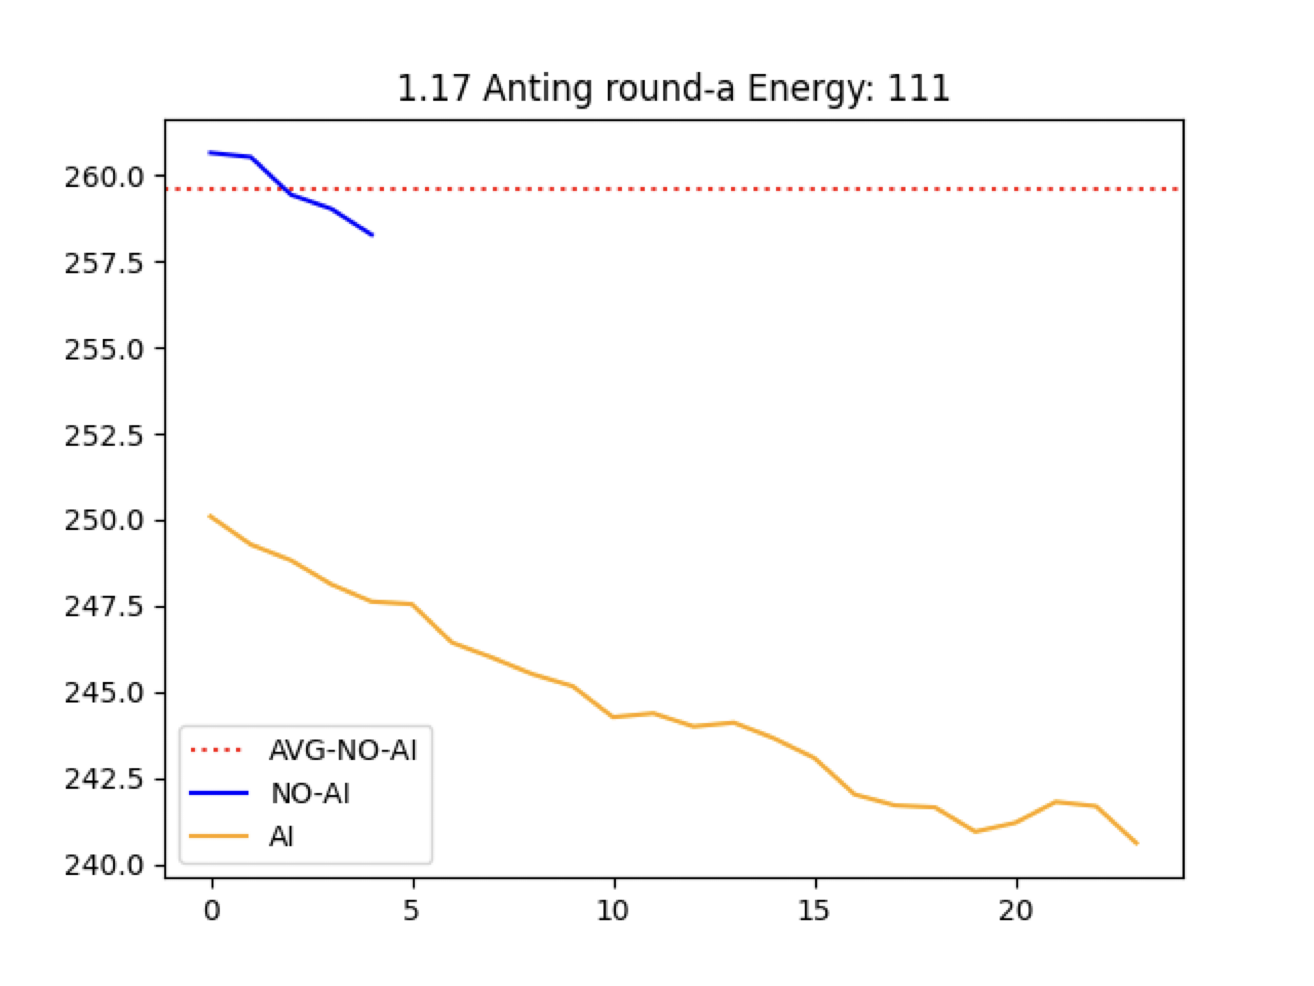
\includegraphics[width=\textwidth]{images/openroad_mm_111_consumption.png}
		\caption{Energy consumption. The reduction is 4.3\% in average.}\label{fig:openroad mm 111 consumption}
	\end{subfigure}
	\hfill
	\begin{subfigure}[t]{0.3\textwidth}
		\centering
		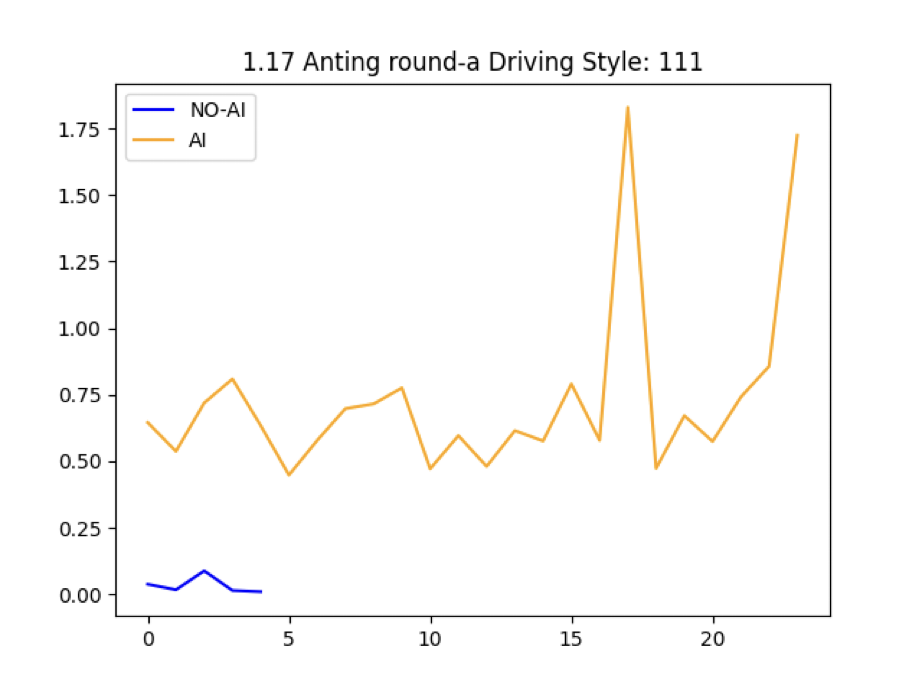
\includegraphics[width=\textwidth]{images/openroad_mm_111_style.png}
		\caption{Driving style drift}\label{fig:openroad mm 111 style}
	\end{subfigure}
	\caption{Scenarios for halting at all turns\label{fig:open road mm 111}}
\end{figure}

We can see from the results that the agent can learn multimodal policies to deal with different scenarios. This indicates a generalized training on real roads without specific handling of the observation data.


\section{Discussion}
\label{sec:discussion}

%If we regard the pedal map as the policy, then the the action we choose is actually is the score function of the policy.

Unlike in the games or robotics, we cannot leverage simulation to provide large amount to training data and cannot do sim2real techniques to accelerate the learning, because there's no available efficient simulation for electric powertrain and complex road condition. Part of the reason is that modeling the real road condition and electric motor is very difficult or expensive, which is the normal case for most of the real world applications. We have to learn from the real world. Surprisingly,  our experiment shows that the application of deep reinforcement learning is quite sample efficient in the energy optimization system. We only need hundreds of episodes to see a clear improvement trend in the result. We believe it's due to the careful design choice of state, action, reward and the data processing that evade much noise in the state and reward.

An practical advantage of the applicaiton is that system safety and task persistency are not issues like in the robotics \parencite{DBLP:journals_ijrr_IbarzTFKPL21}, since the optimiztion of improving energy efficiency is almost not safety relevant. The agent is free to explore diverse strategies with the safeguard of powertrain controlller unit. Failing to reduce the energy consumption will never interrupt the episode, thus the training is reliable, stable and efficient.

In the exeperiment the DDPG policy is short-term with only several seconds of observation. The results match the experience that good human drivers usually don't need long-term strategy to make the right decision for acceleration or braking. However, long-term observations benefit the right decision. For ramps or diffrent topographies of road surfaces which take more than 3 seconds to pass through, the DDPG agent with the current short attention span will not be able to have an optimal policy. To deal with this partial observability, an RDPG agent \parencite{heess15:_memor} is implemented with the LSTM networks \parencite{Hochreiter_1997}. With truncated BPTT \parencite{sutskever2013training} and the stateful feature of LSTM cell \parencite{chollet2015keras}, we can handle arbitrary ragged episode lengths and do inference efficiently with long and short term policies.

The result of transferablitiy in Sec.\@\ref{sec:transferable} with frozen model indicates that while the training must be episodic in order to have meaningful reward signals, the inference-only mode doesn't need to be episodic. A trained frozen model can be deployed for non-episodic situations in inference-only mode in a wide range of applicaitions without the episodic constraint.

The data in Tab.\@\ref{tab:quadruple} has a low density and is light-weight for collection and storage. In order to leverage the large volume of offline data with ongoing training, an offline reinforcement learning is implemented with IDQL \parencite{hansen-estruch23:_idql}. With the offline data, training can occur in the cloud with uploaded observation data from vehicles. The updated local model can be dispatched onto the vehicle through OTA communication. In this framework, the training and inference can be done flexibly either locally or in the cloud, see Fig.\@\ref{fig:Software overview}. Training and inference locally are fast, have better realtime performance and signal quality, but need extra compute resources on the vehicle. The DDPG agent has a size of less than 1MB as exported tflite models which can be easily stored on the embedded system and used in inference, while it's still difficult to accommodate the RDPG agent with its nearly 100 MB on most of the current embedded system in production.\ On the cloud it's more scalable, doesn't need much compute locally but OTA communication with less realtime performance, larger signal latency and lower signal quality. In large scale deployment, training and inferrence on the cloud also provide an opportunity for utilization of parallel training of asynchronous poclicy gradient methods \parencite{mnih16:_async_method_deep_reinf_learn} or federated learning \parencite{konečný15:_feder_optim}.

Diffusion models have been studied actively in recent offine RL researches, in particular in behavior cloning for policy learning \parencite{janner22:_plann_diffus_flexib_behav_synth} \parencite{wang22:_diffus_polic_expres_polic_class} and \parencite{hansen-estruch23:_idql} \parencite{psenka23:_learn_diffus_model_polic_rewar}. Besides utilized by the offline reinforcement learning, the diffusion models can be used to recover complex and multimodal behavior data. With the diffusion model to fit the behavior policy, the drift of the driving style in Fig.\@\ref{fig:openroad a style} is expected to be better tracked by the implicit actor with policy extraction \parencite{hansen-estruch23:_idql}. However, the training and sampling in diffusion models require extra noising and denoising time steps, which reduce its realtime performance and constrains their application. All these improvements require more compute resources and need further verification with large scale deployment.

\section{Conclusion}\label{sec:conclusion}

We present the application of deep reinforcement learning in the optimization of energy efficiency of driving an electric vehicle. We demonstrate that the design choice of the state, reward and action is crucial. If the reward is rich and dense, the application in real world should be sample efficient. If the observation data are of low density and generally accessible like vehicle speed, acceleration and braking pedal opening but contain complex behaviors or system models, we could harvest a large volume of offline data leverage the offline reinforcement learning to improve the optimization process. As reward-driven learning methods are machine learning method which requires no supervision or labeling, but learns from large amount of raw data, they are appealing to the industrial applications. Our experiment is still far from being scaled up. With deployment with large amount of vehicles in the future, we hope to track complex system dynamics, road scenarios and driving behaviors by more efficient RL methods.

The purpose of our work is twofold. On the engineering side, we hope to advocate in the industry to leverage abundant available online or offline domain data and interfaces to achieve continuous and dynamic optimization in complex industrial processes which require the large capacity of deep neural networks and have the potential to help reshaping the industry into the data-driven paradigm.

For research, we intend to provide an application of deep reinforcement learning in the real world that provides interesting and challenging optimization goals. Unlike games or robotics, we cannot always leverage simulation in the real world, but we can have abundant data and achieve sample efficiency with prudent design choice of state, action and reward and by careful implementation which maintains the signal causality and avoids adding noise to state and reward signal. Furthermore, system and task persistency are sometimes guaranteed. More importantly, with large scale deployment of data-driven method and the improvement of the industrial process optimization, a virtuous cycle would contribute to providing abundant data, applying new research results and finding new interesting research challenges.

\begin{appendices}

	\section{System design of EOSEV}\label{sec:system design}

	The EOSEV system consists of four components. Fig.\@\ref{fig:EOSEV system} depict the mode where both training and inference are in the cloud. The environment include the real road and the driver. The environment has an impact on the vehicle which change the vehicle speed, acceleration, brake pedal. The powertrain controller (ECU) collects the energy consumption data synchronously. Then the state and reward are uploaded with timestamps in realtime through telematics box (TBox) and OTA to the database in the cloud, where the agent weights are updated and the action $\Delta\tau$ (parameter optimization) is send back through OTA and TBox to reach the ECU. The ECU updates the pedal map and flashes it into its persistent memory.

	If the ECU or TBox has compute resource, the inference could also happen in the vehicle. In this case, the agent is located in ECU or TBox. The cloud server will send the updated weights of the agent instead of the action, if the training is still in the cloud.

	\begin{figure}[ht]
		\centering
		\def\svgwidth{0.8\columnwidth}
		\input{images/veos_system.pdf_tex}
		\caption{\label{fig:veos} EOSEV system}\label{fig:EOSEV system}
	\end{figure}

	\section{dataflow}\label{sec:dataflow}

	The implementation for the EOSEV is contained in \textbf{tspace} \parencite{github:tspace}. It is an data pipleline framework for deep reinforcement learning with IO interface, processing and configuration. The current code base depicts an automotive implementation. The goal of the system is to increase the energy efficiency (reward) of a BEV by imposing modification on parameters (action) of powertrain controller, the VCU, based on observations of the vehicle (state), i.e.\ speed, acceleration, electric engine current, voltage etc. The main features are:
	\begin{itemize}
		\item both training and inferrence mode;
		\item coordinated ETL and ML pipelines;
		\item both online and offline training,
		\item local and distributed training;
		\item multiple models: with DDPG and RDPG for time sequences with arbitrary length;
		\item offline reinforcement learning with “Implict Diffusion Q-Learning” (IDQ);
		\item compatible data pipelines to both ETL and ML dataflow;
		\item multiple data sources (local CAN or remote cloud object storage);
		\item stateful time sequence processing with sequential model;
		\item support of both NoSQL database, local and cloud data storage.
	\end{itemize}

	The diagram shows the basic architecture.
	\begin{figure}[ht]
		\centering
		\def\svgwidth{0.6\columnwidth}
		% Data flow diagram
% Author: David Fokkema
\documentclass{standalone}
\usepackage{tikz}
\usetikzlibrary{arrows,quotes,shapes.multipart,arrows.meta,matrix,shapes.geometric,backgrounds}

% Defines a `datastore' shape for use in DFDs.  This inherits from a
% rectangle and only draws two horizontal lines.
\makeatletter
\pgfdeclareshape{datastore}{
  \inheritsavedanchors[from=rectangle]
  \inheritanchorborder[from=rectangle]
  \inheritanchor[from=rectangle]{center}
  \inheritanchor[from=rectangle]{base}
  \inheritanchor[from=rectangle]{north}
  \inheritanchor[from=rectangle]{north east}
  \inheritanchor[from=rectangle]{east}
  \inheritanchor[from=rectangle]{south east}
  \inheritanchor[from=rectangle]{south}
  \inheritanchor[from=rectangle]{south west}
  \inheritanchor[from=rectangle]{west}
  \inheritanchor[from=rectangle]{north west}
  \backgroundpath{
    %  store lower right in xa/ya and upper right in xb/yb
    \pgfset{outer xsep=1.5cm}
    \pgfset{outer ysep=1.5cm}
    \southwest \pgf@xa=\pgf@x \pgf@ya=\pgf@y
    \northeast \pgf@xb=\pgf@x \pgf@yb=\pgf@y
    \pgfpathmoveto{\pgfpoint{\pgf@xa}{\pgf@ya}}
    \pgfpathlineto{\pgfpoint{\pgf@xb}{\pgf@ya}}
    \pgfpathmoveto{\pgfpoint{\pgf@xa}{\pgf@yb}}
    \pgfpathlineto{\pgfpoint{\pgf@xb}{\pgf@yb}}
 }
}
\makeatother

\tikzset{
  database_plate/.style={
    cylinder,draw,rotate=90,minimum width=1.5cm,path picture=
    {
      \draw (path picture bounding box.160) to[out=180,in=180,looseness=0.3] (path picture bounding box.20);
      \draw (path picture bounding box.200) to[out=180,in=180,looseness=0.3] (path picture bounding box.340);
    }
  },
  database/.style={
    cylinder,shading=axis,shading angle=0,top color=yellow!10,bottom color=yellow!60,draw,rotate=90,minimum width=1.5cm
  }
}

\begin{document}
\begin{tikzpicture}[
  font=\sffamily,
  every matrix/.style={ampersand replacement=\&,column sep=2cm,row sep=2cm},
  hw/.style={draw,thick,minimum width=2cm,minimum height=1cm,rounded corners,fill=yellow!20,inner sep=.3cm},
  process/.style={draw,thick,circle,fill=blue!20},
  multimodal/.style={circle split,draw,double,fill=blue!20,font=\sffamily\tiny},
  sink/.style={hw,fill=green!20},
  datastore/.style={draw,very thick,shape=datastore,inner sep=.3cm},
  dots/.style={gray,scale=2},
  to/.style={->,>=stealth',shorten >=1pt,semithick,font=\sffamily\footnotesize},
  every edge/.style={draw,>=stealth,shorten <=1pt, shorten >=1pt,semithick,font=\sffamily\footnotesize},
  every edge quotes/.style={auto=left,sloped,font=\sffamily\small},
  every node/.style={align=center}
]
  %every edge/.style={->,>=stealth',shorten >=1pt,semithick,font=\sffamily\footnotesize},
  % Fill the background


  % Position the nodes using a matrix layout
  \matrix (m) [matrix of nodes,
      row sep = 2em, column sep = 2em,
      minimum size=2cm]{
    |[multimodal,rotate=90] (cl)| {
      Cloud OSS \nodepart{lower}
    } RemoteCAN
    \& |[database] (db)| {Storage}
    \& |[process] (mo)| {Model} \\
    |[process] (av)| {Avatar}
    \& |[process] (cr)| {Cruncher}
    \& |[process] (ag)| {Agent} \\
    |[multimodal] (kv)| {
      KvaserCAN
      \nodepart{lower}
    } CAN/UDP server
    \&
    \& \\
    |[hw] (v)| {ECU} \&  \&\\
  };

  % Draw the arrows between the nodes and label them.
  \draw (cr.2) edge [arrows={-Stealth[harpoon]},"observation\\\texttt{\string[Dataframe\string]}",midway,align=center] (ag.178)
        (ag.182) edge [arrows={-Stealth[harpoon]},"\texttt{\string[Dataframe\string]}\\action"',midway,align=center] (cr.358);
  \draw (kv.47) edge [arrows={-Stealth[harpoon]},"Pipeline\\\texttt{\string[json/Dataframe\string]}",midway,align=center] (cr.223)
        (cr.227) edge [arrows={-Stealth[harpoon]},"\texttt{\string[Dataframe/json\string]}\\Pipeline"',midway,align=center] (kv.43);
  \draw (cl.227) edge [arrows={-Stealth[harpoon]},"Pipeline\\\texttt{\string[json/Dataframe\string]}",midway,align=center] (cr.133)
        (cr.137) edge [arrows={-Stealth[harpoon]},"\texttt{\string[Dataframe/json\string]}\\Pipeline"',midway,align=center] (cl.223);
  \draw (db.227) edge [arrows={-Stealth[harpoon]},"Batches\\\texttt{\string[Dataframe\string]}",midway,align=center] (ag.133)
        (ag.137) edge [arrows={-Stealth[harpoon]},"\texttt{\string[Dataframe\string]}\\Episode"',midway,align=center,pos=0.6] (db.223);
  \draw (ag.92) edge [arrows={-Stealth[harpoon]},"observation\\\texttt{\string[Dataframe\string]}",midway,align=center] (mo.268)
        (mo.272) edge [arrows={-Stealth[harpoon]},"action\\\texttt{\string[Dataframe\string]}",midway,align=center] (ag.88);
  \draw (ag.0) edge [->,bend right,"\texttt{\string[Dataframe\string]}\\Batches"',midway,align=center] (mo.0);
  \draw (mo) edge[->,loop left,out=225,in=135, looseness=5] node[font=\sffamily\small,right]{Train} (mo);
  \draw (av.2) edge [->,dotted,"config." above,"sched." below,font=\sffamily\tiny] (cr.178);
  \draw (kv) edge [<-,dotted,"config." above,"sched." below,font=\sffamily\tiny] (av);
  \draw (av) edge [->,dotted,"config." above,"sched." below,font=\sffamily\tiny] (cl);
  \draw (v) edge [<->,"CAN" above, "UDP" below] (kv);
  \draw (cl.137) edge [<->, densely dash dot dot,bend right,"OTA"] node[hw,minimum width=1cm,minimum height=0.5cm,solid,very near end, sloped,]{TBox} (v.133);

  % Background rectangle
    \begin{scope}[on background layer]
        \fill[green!10] (current bounding box.south west) rectangle (current bounding box.north east);
    \end{scope}
\end{tikzpicture}
\end{document}

		\caption{\label{fig:Software overview} Software Overview}
	\end{figure}
	The dataflow of the pipelines
\end{appendices}
%\bibliographystyle{unsrtnat}
%\bibliographystyle{abbrvnat}
%%% Uncomment this section and comment out the \bibliography{references} line above to use inline references.
% \begin{thebibliography}{1}

% 	\bibitem{kour2014real}
% 	George Kour and Raid Saabne.
% 	\newblock Real-time segmentation of on-line handwritten arabic script.
% 	\newblock In {\em Frontiers in Handwriting Recognition (ICFHR), 2014 14th
% 			International Conference on}, pages 417--422. IEEE, 2014.

% 	\bibitem{kour2014fast}
% 	George Kour and Raid Saabne.
% 	\newblock Fast classification of handwritten on-line arabic characters.
% 	\newblock In {\em Soft Computing and Pattern Recognition (SoCPaR), 2014 6th
% 			International Conference of}, pages 312--318. IEEE, 2014.

% 	\bibitem{keshet2016prediction}
% 	Keshet, Renato, Alina Maor, and George Kour.
% 	\newblock Prediction-Based, Prioritized Market-Share Insight Extraction.
% 	\newblock In {\em Advanced Data Mining and Applications (ADMA), 2016 12th International
%                       Conference of}, pages 81--94,2016.

% \end{thebibliography}

\printbibliography

\end{document}
